\documentclass{article}

\usepackage{amsmath, amsthm, amssymb, amsfonts}
\usepackage{thmtools}
\usepackage{graphicx}
\usepackage{setspace}
\usepackage{geometry}
\usepackage{float}
\usepackage{hyperref}
\usepackage[utf8]{inputenc}
\usepackage[english]{babel}
\usepackage{framed}
\usepackage[dvipsnames]{xcolor}
\usepackage{tcolorbox}
\usepackage{pgfplots}
\usepackage{tikz}
\usepackage{enumitem}
\pgfplotsset{compat=1.18}

\colorlet{LightGray}{White!90!Periwinkle}
\colorlet{LightOrange}{Orange!15}
\colorlet{LightGreen}{Green!15}

\newcommand{\HRule}[1]{\rule{\linewidth}{#1}}

\declaretheoremstyle[name=Teorema,]{thmsty}
\declaretheorem[style=thmsty,numberwithin=section]{theorem}
\tcolorboxenvironment{theorem}{colback=LightGray}

\declaretheoremstyle[name=Ejercicio,]{prosty}
\declaretheorem[style=prosty,numberlike=theorem]{exercise}
\tcolorboxenvironment{exercise}{colback=LightOrange}

\declaretheoremstyle[name=Demostración,]{prcpsty}
\declaretheorem[style=prcpsty,numberlike=theorem]{proofs}
\tcolorboxenvironment{proofs}{colback=LightGreen}

\pgfmathdeclarefunction{gauss}{2}{\pgfmathparse{1/(#2*sqrt(2*pi))*exp(-((x-#1)^2)/(2*#2^2))}}

\setstretch{1.2}
\geometry{
    textheight=9in,
    textwidth=5.5in,
    top=1in,
    headheight=12pt,
    headsep=25pt,
    footskip=30pt
}

% ------------------------------------------------------------------------------

\begin{document}

% ------------------------------------------------------------------------------
% Cover Page and ToC
% ------------------------------------------------------------------------------

\title{ \normalsize \textsc{}
\\ [2.0cm]
\HRule{1.5pt} \\
\LARGE \textbf{\uppercase{Inferencia Estadística II}
\HRule{2.0pt} \\ [0.6cm] \LARGE{Tema 1: Propiedades asintóticas del EMV y del estadístico RV} \vspace*{10\baselineskip}}
}

\author{\textbf{Autores} \\
    Victor Elvira Fernández, Tomás Ruiz Rojo, Juan Horrillo Crespo \\
    Universidad de Valladolid \\
    \date{\today}}

\maketitle
\newpage

\begin{center}
    \Huge \textbf{AVISO}
\end{center}

Estos apuntes fueron creados de forma voluntaria por un grupo de estudiantes, invirtiendo tiempo, dedicación y esfuerzo para ofrecer información útil a la comunidad. Apreciamos cualquier apoyo que se nos quiera brindar, ya que nos ayuda a continuar con futuros proyectos de este tipo. \\

Si deseas colaborar en esta clase de proyectos puedes contactarnos y unirte o invitarnos a unas ricas patatas 5 salsas por el siguiente enlace:

\vfil

\begin{center}
    \href{https://www.buymeacoffee.com/ApuntesINdat}{\LARGE \textbf{Buy Me a Patatas 5 Salsas}}
    \href{https://www.buymeacoffee.com/ApuntesINdat}{https://www.buymeacoffee.com/ApuntesINdat}
\end{center}

\begin{itemize}
    \item \href{mailto:juan.horrillo22@estudiantes.uva.es}{Mail Juan Horrillo}
    \item \href{mailto:victor.elvira22@estudiantes.uva.es}{Mail Victor Elvira}
    \item \href{mailto:tomas.rojo22@estudiantes.uva.es}{Mail Tomás Rojo}
\end{itemize}

\vfil

Si has colaborado de cualquier forma te agradecemos enormemente.

\tableofcontents
\newpage

% ------------------------------------------------------------------------------

% \section{Propiedades asintóticas del EMV y del estadístico RV xd}


\subsection{Estimadores en muestras grandes}

Nuestro principal objetivo es analizar cómo se comporta la muestra cuando su tamaño es tan grande como nosotros queramos.
\setlength{\parskip}{1em}   % Aumentar espacio entre párrafos

Situación:
\setlength{\parskip}{0em}   % Aumentar espacio entre párrafos

\( X_1, X_2, \dots, X_n \) variables aleatorias independientes igualmente distribuidas (v.a.i.i.d.) tal que \( P_\theta:\theta  \in  \Theta\).

Tenemos nuestra muestra aleatoria simple (m.a.s) con \( n \) grande y nos interesa estimar \( \theta \) (o \( g(\theta) \)).

\setlength{\parskip}{1em}   % Aumentar espacio entre párrafos
Cuando el tamaño de la muestra aumenta, también aumenta la información disponible de \( \theta \) (o \( g(\theta) \)), por lo tanto se espera que la estimación sea más precisa.

Si tenemos un estimador \( T(X_1, \dots, X_n) \) razonable, cuando \( n \) aumenta, el estimador \( T(X_1, \dots, X_n) \) deberá ser más preciso.

\setlength{\parskip}{0em}   % Aumentar espacio entre párrafos
Lo que podemos esperar es que \( T(X_1, \dots, X_n) \) esté próximo a \( \theta \) con mayor probabilidad.

\subsubsection{Consistencia de un estimador}

Se dice que un estimador es consistente si cumple:
\setlength{\parskip}{1em}

\[\forall \epsilon > 0, \; \delta > 0 \quad \exists N: n \geq N\]
\[P_\theta\left(|T(X_1, \dots, X_n) - \theta| < \epsilon\right) \geq 1 - \delta\]

\textbf{\textit{Definición: }} \(T_n(X)\) es un estimador consistente para \(\theta\) (o \(g(\theta)\)) si:

\[
    \forall \epsilon > 0 \quad P_\theta\left(|T(X_1, \dots, X_n) - \theta| \leq \epsilon\right) \xrightarrow{n \to \infty} 1
\]

es decir, si:

\[
    T_n(x) \xrightarrow{\underset{n \to \infty}{\text{P}}} \theta \quad \text{o} \quad \lim_{n \to \infty} \forall \epsilon > 0 \quad P_\theta\left(|T(X_1, \dots, X_n) - \theta| \leq \epsilon\right) = 1
\]

\newpage
\subsubsection*{Estrategias para comprobar si un estimador es consistente}

\begin{enumerate}
    \setlength{\parskip}{1em}
    \item \textbf{Si converge en probabilidad.}
          Resultado:
          \[
              Si \quad T_n(x) \xrightarrow{\underset{n \to \infty}{\text{P}}} \theta \quad \text{y} \quad T_n(x) \xrightarrow{\underset{n \to \infty}{\text{P}}} \theta'
          \]
          \begin{itemize}
              \item \(T_n(x)+G_n(x) \xrightarrow{\underset{n \to \infty}{\text{P}}} \theta + \theta '\)
              \item \(T_n(x)G_n(x) \xrightarrow{\underset{n \to \infty}{\text{P}}} \theta\theta '\)
              \item Si \(\theta' \neq 0, \frac{T_n(x)}{G_n(x)} \xrightarrow{\underset{n \to \infty}{\text{P}}} \frac{\theta}{\theta '}\)
          \end{itemize}

    \item \textbf{Utilizando la ley débil de los grandes números.}
          \(X_1, X_2, \dots, X_n\) i.i.d. con \(E(X_i)=\mu < \infty\)
          \setlength{\parskip}{0em}
          \[\frac{1}{n}\sum_{i=1}^{n} X_i \xrightarrow{\underset{n \to \infty}{\text{P}}} \mu\]

          \setlength{\parskip}{1em}
          Los momentos muestrales son estimaciones consistentes de los correspondientes momentos poblacionales

    \item \textbf{Utilizando la convergencia en media cuadrática.}
          Un estimador $T(X_1, \dots, X_n)\xrightarrow{\underset{n \to \infty}{\text{m.c.}}} \theta$ si:
          \begin{itemize}
              \item \(E(T(X_1, \dots, X_n)) \xrightarrow{{n \to \infty}} \theta\), sesgo(\(T(X_1, \dots, X_n)\)) \(\xrightarrow{{n \to \infty}} 0\)
              \item \(\text{Var}(T(X_1, \dots, X_n)) \xrightarrow{{n \to \infty}} 0\)
          \end{itemize}
          Es decir que si ECM ($T(X_1, \dots, X_n)$) \(\xrightarrow{{n \to \infty}} 0\), el estimador converge en media cuadrática. Un estimador insesgado sería consistente si su varianza converge a 0 con \(n \to \infty\)

          El resultado es que la convergencia en media cuadrática es más fuerte que la convergencia en probabilidad.
\end{enumerate}
\noindent\rule{\textwidth}{0.2pt} % Línea de separación

\subsubsection*{Ejercicio 1}
\(X_1, \dots, X_n \) v.a.i.i.d \quad E(X_i)=\mu, \text{Var}(X_i)=\sigma^2 \quad \forall i=1, \dots, n

¿Es consistente $T_n(x) = \frac{X_1 + X_2 + \dots + X_n}{\frac{n}{2}}$?

Usando la ley de los grandes números:
\(\frac{1}{n}\sum X_i \xrightarrow{\text{P}} \mu \quad T_n(x)\xrightarrow{\text{P}}2\mu\)

Resultado: El estimador \(T_n(x)\) NO es consistente

\newpage

La consistencia por si sola no es tan interesante, ya que si $T_n \text{es consistente para } \theta$, nos dice que para n grande los errores serán pequeños pero no nos permite conocer el orden del error $\left(\frac{1}{n}, \frac{1}{\sqrt{n}},\frac{1}{\log(n)}, \dots\right)$

Si $\{K_n\}_{n=1}^{\infty}$ es una sucesión de reales positivos y $\epsilon>0$ definimos $P_n(\epsilon)$.

\(P_n(\epsilon)=P_\theta(|T_n(x)-\theta| \leq \frac{\epsilon}{K_n})\)

Habiendo definido \(P_n(\epsilon)\), ¿qué pasará con  \(P_n(\epsilon)\) cuando n sea grande?
\begin{enumerate}
    \item Si \(K_n\) crece "lentamente" (por ejemplo:  \(K_n=\log(n)\)), el error disminuye "lentamente" a medida que aumenta n \(P_n(\epsilon) \xrightarrow{{\text{n} \to \infty}} 1\). Si \(K_n\) crece lentamente, \( \frac{\epsilon}{K_n}\) es más grande, lo que facilitará que el error esté por debajo del umbral.
    \item Si \(K_n\) crece "rápido" (por ejemplo:  \(K_n=n\)), el error disminuye más rápido a medida que aumenta n \(P_n(\epsilon) \xrightarrow{{\text{n} \to \infty}} 0\).  Si \(K_n\) crece rápido, \( \frac{\epsilon}{K_n}\) se hace muy pequeño y se hace muy difícil que el error sea tan pequeño.
    \item Casos intermedios.

          Si \(K_n\) crece "adecuadamente", \(P_n(\epsilon) \xrightarrow{{\text{n} \to \infty}} H(\epsilon) \in (0,1)\). Decimos que el error converge a 0 a velocidad \(\frac{1}{K_n}\)
\end{enumerate}
De manera resumida:

\(
P_n(\epsilon) = P_\theta(K_n|T_n(x) - \theta| \leq \epsilon) \xrightarrow{{n \to \infty}

\left\{
\begin{array}{l}
    0 \text{ si } K_n \xrightarrow{\infty} \text{ "rápido"}                                  \\[1em]
    0 \leq P_n(\epsilon) \leq 1 \text{ si } K_n \xrightarrow{\infty} \text{ "adecuadamente"} \\[1em]
    1 \text{ si } K_n \xrightarrow{\infty} \text{ "lento"}
\end{array}
\right\}
\)

La idea es que al multiplicar $K_n$, se amplifica la velocidad de convergencia de los errores a 0. Si elegimos $K_n$ adecuadamente, de forma que $P_n(\epsilon)$ sea menor que 1, podemos controlar la velocidad a la que los errores tienden a 0, mejorando la precisión.

% 
\setlength{\parskip}{1em}
\subsubsection*{Ejercicio 1}

$X_1, \dots, X_n$ v.a.i.i.d. $\quad E(X_i)=\mu,\quad Var(X_i)=\sigma^2 \quad \forall i=1 \dots n$

b) $T(X_1,\dots,X_n)=\frac{T(X_1 + \dots + X_{\frac{n}{2}})}{\frac{n}{2}}$\\
$T(X_1,\dots,X_n) \xrightarrow{P} \mu \quad$ El estimador es consistente

c) $T(X_1,\dots,X_n)=X_1$\\
El estimador no es consistente ya que $X_1$ no depende de n. Lo mínimo para que
pueda converger es que dependa de n.

d) $T(X_1,\dots,X_n)=2 \cdot \sum_{i=1}^{n}\frac{i \cdot X_i}{n \cdot (n+1)}$\\
No podemos usar la ley de los grandes números porque $X_1, 2 \cdot X_2, 3 \cdot X_3$ no son v.a.i.i.d. Usaremos la convergencia en media cuadrática.

\[
T_n(x) \xrightarrow{m.c.} \mu 
\left\{
\begin{array}{l}
    E(T_n(X)) \xrightarrow[n \to \infty]{} \mu \\
    Var(T_n(X)) \xrightarrow[n \to \infty]{} 0
\end{array}
\right.
\]
\(
E(T_n(x))=\frac{2}{n \cdot (n+1)} \cdot E((\sum_{i=1}^{n} i) \cdot X_i)
=\frac{2}{n \cdot (n+1)} \cdot (\sum_{i=1}^{n} i) \cdot  E(X_i)=
\frac{2 \cdot \mu}{n \cdot (n+1)} \cdot \sum_{i=1}^{n} i \\
=\frac{2 \cdot \mu}{n \cdot (n+1)} \frac{n \cdot (n+1)}{2}= \mu
\)

Se cumple que la media tiende a mu cuando n tiende a infinito.

\(
Var(T_n(x))=\frac{4}{n^2 \cdot (n+1)^2} \cdot \sum_{i=1}^{n} Var(i\cdot X_i)
= \frac{4}{n^2 \cdot (n+1)^2} \cdot \sigma^2 \cdot \sum_{i=1}^{n} i^2 \\
= \frac{4}{n^2 \cdot (n+1)^2} \cdot \sigma^2 \cdot \frac{n \cdot (n+1) \cdot (2n+1)}{6}
=\frac{2}{3}\cdot \frac{2n+1}{n^2+n} \sigma^2 \xrightarrow[n \to \infty]{} 0
\)

Se cumple que la media tiende a 0 cuando n tiende a infinito.

El estimador es consistente.

\subsubsection*{Ejercicio 3}

$X_1, \dots, X_n$ v.a.i.i.d. con distribución uniforme U($0,\theta$)

¿$2 \bar{X}$ es consistente para $\theta$?

\(
E(X_i)=\frac{a+b}{2}=\frac{\theta}{2};\quad Var(X_i)=\frac{(b-a)^2}{12}
\)

$\bar{X} \xrightarrow[n \to \infty]{P} \implies 2 \bar{X} \xrightarrow{P} \theta
$

$2 \bar{X}$ es consistente para $\theta$
\newpage

\subsubsection{Información de Fisher}

La información de Fisher $I_x(\theta)$ es la matriz que mide la cantidad
de información que una m.a.s. contiene sobre el estimador.

\textbf{\textit{Definición: }} Sea X=($X_1 \dots X_n$) v.a.i.i.d. con distribución
$P_\theta \in P=\{P_\theta : \theta \in \Theta \subseteq \mathbb{R}\}$
con función de densidad f(X,$\theta$) y en la que existe $\frac{d f(x,\theta)}{d \theta}$
, la información de Fisher sobre $\theta$ contenida en X es:
\[
I_x(\theta) = Var_\theta (S(\theta,X))
\]
\[
Score=S_x(\theta)=S(\theta,X)=\frac{d}{\mathrm{d\theta}}
\log f(x,\theta)
\]
\subsubsection{Condiciones de regularidad de Craner-Rao (CRCR)}

Llamaremos familias regulares a aquellas familias en las que se verifican las 
condiciones de regularidad de Craner-Rao.
\\ Estas son las familias con las que trabajaremos.

\textbf{Condiciones de regularidad de Craner-Rao:}
\begin{enumerate}
    \item El espacio paramétrico es un intervalo de $\mathbb{R}$.
    \item El soporte de la distribución no depende del parámetro $\theta$.
    
    Por ejemplo $x=\{x:f(x,\theta) > 0 \}$, no depende de $\theta$ y sería regular. En cambio U(0,$\theta$) 
    tiene un soporte que depende de $\theta$, por lo que no es regular
    \item Se pueden calcular las dos primeras derivadas bajo el signo integral.
     Además se puede intercambiar la derivada con el signo integral.
     
    \(
    \frac{d}{d \theta} \int_{x} f(x,\theta)  \,dx =
    \int_{x} \frac{d}{d \theta} f(x,\theta)  \,dx
    \)
    \item $T_n(x)$ es un estimador insesgado para $\theta$ o $g(\theta)$.
\end{enumerate}

Bajo las condiciones de regularidad de Craner-Rao, podemos definir la cantidad
de información esperada como:
\[
I_x(\theta)=E_\theta(S(\theta,X)^2)=E_\theta((\frac{d}{d \theta} \log f(x,\theta))^2)
\]
\textbf{\textit{Demostración:}}
Deberemos probar que $E_\theta((\frac{d}{d \theta} \log f(x,\theta)))=0$.
Si lo conseguimos probar entonces, $Var(S(\theta,x))=E(S(\theta,x)^2)
-E(S(\theta,x))^2=E(S(\theta,x)^2)$

\(
    E_\theta((\frac{d}{d \theta} \log f(x,\theta)))=
    \int_{x} E_\theta((\frac{d}{d \theta} \log f(x,\theta))) \cdot f(x,\theta) \,dx 
    =\int_{x} \frac{\frac{d}{d \theta} f(x,\theta)}{f(x,\theta)} \cdot f(x,\theta) \,dx 
    \\=\int_{x} \frac{d}{d \theta} f(x,\theta) \,dx = 0
\)

Si se verifican las condiciones de regularidad de Crner-Rao, otra forma alternativa de calcular
la información de Fisher es:
\[
I_x(\theta)=-E(\frac{d^2}{d \theta} \log f(x,\theta))
\]

\textbf{\textit{Demostración:}}

Breve paso previo:


\(
\frac{d}{d \theta} (\frac{d}{d \theta} \log f(x,\theta))=
\frac{d}{d \theta} (\frac{\frac{d}{d \theta} f(x,\theta)}{f(x,\theta)})
\text{= (derivando el cociente)}
\frac{\frac{d^2}{d \theta} f(x,\theta) f(x,\theta) - (\frac{d}{d \theta} f(x,\theta))^2}{f(x,\theta)^2}
\\ = \frac{\frac{d^2}{d \theta} f(x,\theta)}{f(x,\theta)} - (\frac{\frac{d}{d \theta} f(x,\theta)}{f(x,\theta)})^2
\)

Demostración:

\(
E(\frac{d^2}{d \theta} \log f(x,\theta))=
\int_{x} frac{d}{d \theta} (\frac{d}{d \theta} \log f(x,\theta)) \cdot f(x,\theta) \,dx = \\
\int_{x} \frac{d^2}{d \theta} f(x, \theta) \,dx - \int_{x} (\frac{\frac{d}{d \theta} f(x,\theta)}{f(x,\theta)})^2 \cdot f(x,\theta) \,dx  
= - \int_{x} (\frac{\frac{d}{d \theta} f(x,\theta)}{f(x,\theta)})^2 \cdot f(x,\theta) \,dx  
= - I_x(\theta)
\)

\textbf{\textit{Propiedades:}}

Sean X e Y dos variables independientes de la misma familia de distribuciones.

$
X \sim P_\theta, \quad \theta \in \Theta \subseteq \mathbb{R}, \quad f(x,\theta), I_x(\theta)
$
$
Y \sim Q_\theta, \quad \theta \in \Theta \subseteq \mathbb{R}, \quad g(y,\theta), I_y(\theta)
$

% \setlength{\parskip}{1em}

Vamos a profundizar un poco en las condiciones de regularidad de Craner-Rao:

Sea X=$(X_1,\dots,X_n)$ m.a.s de $P_\theta,\theta \in \Theta \subseteq \mathbb{R}$
,con densidad f(x,$\theta)$ y con $T_n(x)$ como estimador insesgado de g($\theta$).

\[
E(T_n(x)=g(\theta)) \to g(\theta)=\int_x T_n(x) f(x,\theta) \,dx
\]

$g(\theta)$ es diferenciable resoecto a $\theta$ bajo el signo integral y podemos intercambiar derivada e integral

\subsection{Cota de Craner-Rao}

Sea $X_,\dots,X_n$ m.a.s $P_\theta,\theta \in \Theta \subseteq \mathbb{R}$ con densidad
$f(x,\theta)$ y sea $T_n(x)$ un estimador insesgado de $g(\theta)$ con Var$(T_n(x)) < \infty$
y que verifica las condiciones de regularidad de Craner-Rao, entonces:
\[
Var(T_n(x)) \geq \frac{(g'(\theta))^2}{n \cdot I_{x_1}(\theta)}
\]

\textbf{Demostración:}

Consideremos $Cov(T_n(x),S_x(\theta))=E(T_n(x)\cdot S_x(\theta))$

\(
\\ Cov(T_n(x)S_x(\theta))=\int_x T_n(x) \cdot S_x(\theta) \cdot f(x,\theta) \,dx
=\int_x T_n(x) \cdot \frac{d}{d \theta} \log f(x,\theta) \cdot f(x,\theta) \,dx
\\=\int_x T_n(x) \cdot \frac{\frac{d}{d \theta f(x,\theta)}}{f(x,\theta)} \cdot f(x,\theta) \,dx
=\int_x T_n(x) \cdot \frac{d}{d \theta} f(x,\theta)\,dx
= \frac{d}{d \theta} \int_x T_n(x) f(x,\theta) \,dx
=\frac{d}{d \theta} E(T_n(x))
\\ \text{(Como }T_n(x) \text{ es insesgado:)}
\\ =\frac{d}{d \theta} g(\theta)=g'(\theta)
\)

Usamos la desigualdad de Cauchy-Schwarz que relaciona varianza y covarianza 

$cov(X,Y)=\sqrt{Var(X) \cdot Var(Y)}$

entonces,

\(
(g'(\theta)^2)=(cov(T_n(x)\cdot S_x(\theta)))^2 \leq Var(T_n(x)) \cdot Var(S_x(\theta))
=Var(T_n(x)) \cdot n \cdot I_{x_1}(\theta)
\)

\[
Var(T_n(x)) \geq \frac{(g'(\theta))^2}{n \cdot I_{x_1}(\theta)}
\]

La varianza de un estimador insesgado es como mínimo $\frac{(g'(\theta))^2}{n \cdot I_{x_1}(\theta)}$

Nota: Bajo las mismas condiciones de regularidad de Craner-Rao puede estiamrse
en el caso que $T_n(x)$ sea un estimador de $\theta$ con $Var(T_n(x))<\infty$

\[
Var(T_n(x)) \geq \frac{1}{n \cdot I_{x_1}(\theta)}= \frac{1}{I_n(\theta)}
\]


La demostración es anaáloga a la anterior.

\subsubsection*{Ejemplo}


\(
X_1,\dots,X_n \sim B(p) \quad p \in (0,1)
\\I_n(\theta)=n \cdot I_{x_1}(\theta)=\frac{n}{p(1-p)}
\)

Si quiero estimar p, ¿cuál es la cota CR para cualquier estimador insesgado de P?

\(
Var(T_n(x)) \geq \frac{1}{n \cdot I_{x_1}(p)}=\frac{p(1-p)}{n}
\)

Supongamos que nuestro estimador para p es $\bar{X}$

$Var(\frac{\sum_{i=1}^{n}}{n})=\frac{1}{n^2}Var(\sum_{i=1}^{n} x_i)
=\frac{n \cdot p(1-p)}{n^2}=\frac{p(1-p)}{n}$

\noindent\rule{\textwidth}{0.5pt} % Línea de ancho completo y grosor ajustado

Hemos visto que,como consecuencia del Teorema Central del Limite,  la velocidad de convergencia de los errores a cero es del orden $\frac{1}{\sqrt{n}}$

Si $X_1,\dots,X_n$ i.i.d. $P_\theta \in P,\theta \in \Theta \subseteq \mathbb{R}$ y f($x,\theta$)
verifica las condiciones de regularidad de Craner-Rao, es decir, si la familia es regular.

$\sqrt{n}(T_n(x)-g(\theta)) \xrightarrow{L} N(0,V_T^2(\theta))$

donde $V_T^2(\theta)$ es la varianza asintótica del estimador y $\sqrt{n}$ es la normalización
adecuada como consecuencia del TCL.

Es equivalente, $T_n(x) \simeq N(g(\theta),\frac{V_T^2(\theta)}{n})$

Bajo esas condiciones de regularidad, la varianza $\frac{V_T^2(\theta)}{n}$
cumple también la cota de Craner-Rao

\subsubsection*{Ejemplo:}

\(
X_1,\dots,X_n \quad i.i.d \quad U(0,\theta) \quad \theta>0
\\f(x,\theta)= \frac{1}{\theta} \quad
\)
(Ejercicio 3b)

Se demuestra que $X_{(n)}$ es un estimador consistente para $\theta$, pero la velocidad de convergencia no es $\frac{1}{\sqrt{n}}$

\subsection{Estimador Consistente Asintóticamente Normal (CAN) y \texorpdfstring{\\}{ } Asintóticamente Eficiente (AE)}

Sea $X_1,\dots,X_n$ m.a.s. de $P_\theta, \theta \in \Theta \subseteq \mathbb{R}$
 con densidad $f(x,\theta)$ y $T_n(x)$ estimador insestado de g($\theta$) con una Var($T_n(x))<\infty$
 y que verifica las condiciones de regularidad DE Craner-Rao, entonces:

\[
Var(T_n(x)) \geq \frac{(g'(\theta))^2}{n \cdot I_{x_1}(\theta)}
\]

,es decir,

\[
\frac{V_T^2(\theta)}{n} \geq \frac{(g'(\theta))^2}{n \cdot I_{x_1}(\theta)}
\]
\[
V_T^2(\theta) \geq \frac{(g'(\theta))^2}{I_{x_1}(\theta)}
\]

Concretamente un estimador CAN será mejor cuanto menor sea la varianza asintótica. 
Si la varianza del estimador original es igual a la cota de CRaner-Rao, decimos que $T_n(x)$ es CAN y asintóticamente eficiente (AE)

\textbf{\textit{Definición: }}$X_1,\dots,X_n$ m.a.s.$P_\theta, \theta \in \Theta \subseteq \mathbb{R}, f(x,\theta), T_n(x)$
es un estimador CAN y AE de g($\theta$) si es CAN y $V_T^2=\frac{(g'(\theta))^2}{I_{x_1}(\theta)}$, es decir si
\[
\sqrt{n}(T_n(x)-g(\theta))\xrightarrow{L}N(0,\frac{(g'(\theta))^2}{I_{x_1}(\theta)})
\]


\subsubsection*{Ejemplo:}

\(
X \sim P(\lambda) \quad \lambda>0 \quad f(x,\theta)=\frac{e^{-\lambda}\cdot \lambda^x}{x!} \quad x=0,1,2,\dots
\\ E(X)=\lambda \quad Var(X)=\lambda
\\ \log F(x,\theta)=-\lambda + x \cdot \log \lambda - \log x!
\)

Buscamos un estimador CAN y AE para $\lambda$.

Por el teorema central del límite, la media muestral es CAN para la media poblacional.

\(
\sqrt{n}(\bar{X}-\lambda) \xrightarrow{L} N(0,\lambda)
\quad o \quad \bar{X} \simeq N(\lambda,\frac{\lambda}{n})
\)

Para comprobar si $\bar{X}$ es AE, debemos comprobar que $\frac{\lambda}{n}$ es igual a $\frac{1}{n \cdot I_{x_1}(\lambda)}$

\(
S_x(\lambda)=\frac{x-\lambda}{\lambda} \quad I_{x_1}=\frac{1}{\lambda}
\)

La varianza de $\bar{X}$ coincide con la cota de Craner-Rao, por lo que es un estimador
$\\$ asintóticamente eficiente
($\frac{1}{n\cdot I_{x_1}(\lambda)}=\frac{1}{n\cdot \frac{1}{\lambda}}=\frac{\lambda}{n}$)

\subsubsection*{Ejemplo:}

\(
X \sim exp(\lambda) \quad f(x,\lambda)=\lambda \cdot e^{-\lambda \cdot x} \quad x>0, \quad \lambda>0
\\ E(X) = \frac{1}{\lambda} \quad Var(X)=\frac{1}{\lambda^2}
\\ \log f(x,\lambda)= \log \lambda - \lambda \cdot X
\\ S(\lambda,x)=\frac{1}{\lambda}-X
\\ \sqrt{n}(\bar{X}-\frac{1}{\lambda}) \xrightarrow{L} N(0,\frac{1}{\lambda^2})
\\ \bar{X} \simeq N(\frac{1}{\lambda},\frac{1}{n \cdot \lambda^2})
\)

Sabemos que $\bar{X}$ es CAN para $\frac{1}{\lambda}$, es decir para
$g(\lambda)=\frac{1}{\lambda} ;  g'(\lambda)=\frac{-1}{\lambda^2}$
.

Queremos ver si tambien es AE para la media poblacional. Tenemos que comprobar que $\frac{V_T^2(\lambda)}{n}=\frac{1}{\lambda^2}$
coincida con la cota CR.

\(
I_{x_1}=\frac{1}{\lambda^2} \quad \frac{(g'(\theta))^2}{n \cdot I_{x_1}(\theta)}=
\frac{(\frac{-1}{\lambda^2})^2}{n \cdot \frac{1}{\lambda^2}}=\frac{1}{n \cdot \lambda^2}
\)

¿Y como obtendríamos un estimador AE para $\lambda$?
Utilizando el delta método.

Si $T_n(x)$ es CAN para $\theta \in \Theta \subseteq \mathbb{R}$ y g es una función con derivada no nula, 
entonces $g(T_n(x))$ es CAN para $g(\theta)$ con varianza $\frac{V_T^2}{n}\cdot (g'(\theta))^2$

$\sqrt{n}(T_n(x)-\theta) \xrightarrow{L}N(0,V_T^2(\theta))$

$\sqrt{n}(g(T_n(x))-g(\theta)) \xrightarrow{L} N(0,V_T^2(\theta)\cdot(g'(\theta))^2)$

Volviendo al ejemplo, tras esta breve parte teórica, ya vimos que $\sqrt{n}(\bar{X}-\frac{1}{\lambda})\xrightarrow{L} N(0,\frac{1}{\lambda})$.
Consideraremos que $\theta=\frac{1}{\lambda^2}$.

Pasos:
\begin{enumerate}
    \item $\sqrt{n}(\bar{X}-\theta)\xrightarrow{L}N(0,\theta^2)$
    \item Delta método:
    \(
    \\ g(\theta)=\frac{1}{\theta} \quad;\quad g'(\theta)\frac{-1}{\theta^2}
    \\ \sqrt{n}(g(\bar{X})-g(\theta)) \xrightarrow{L} N(0,\theta^2(\frac{-1}{\theta^2})^2)
    \\ \sqrt{n}(\frac{1}{\bar{X}}-\frac{1}{\theta}) \xrightarrow{L} N(0,\frac{1}{\theta^2}) 
    \)
    \item $ \sqrt{n}(\frac{1}{\bar{X}}-\lambda) \xrightarrow{L} N(0,\lambda^2) \quad o \quad 
    \frac{1}{\bar{X}}\eqsim N(\lambda,\frac{\lambda^2}{n})$
\end{enumerate}

Entonces, $\frac{1}{\bar{X}}$ es CAN para $\lambda$ y $\frac{V_T^2(\lambda)}{n}=\frac{\lambda^2}{n}$

Ahora nos cuestionamos, ¿es $\frac{1}{\lambda}$ AE?

Teniamos que $I_{x_1}(\lambda)=\frac{1}{\lambda^2}$, por lo que la cota CR será $\frac{1}{n \cdot I_{x_1}(\lambda)}=\frac{\lambda^2}{n}$.
Es un estimador asintóticamente eficiente.

\textbf{Resultado: }Todos los estimadores CAN que se obtienen usando el delta método a partir de un estimador asintóticamente eficiente,
son asintóticamente eficientes.

(La demostracción era tarea)

\subsubsection{Estimadores razonables}

Los estimadores CAN y AE son estimadores con propiedades razonables, pero podemos tener más de un estimador razonable.

Sean $T_n(x)$ estimador CAN para g($\theta$) y $G_n(x)$ estimador CAN para g($\theta$)
\begin{itemize}
    \item Si uno de los 2 es AE y el otro no, el estimador AE es mejor.
    \item Si ambos son AE, será mejor el que tenga una menor varianza asintótica($V_T^2$).
\end{itemize}

Para ver cual tiene una menor varianza asintótica, usamos la eficiencia relativa asintótica.

\textbf{\textit{Definición: }} $X_1,\dots,X_n$ i.i.d. $\{ P_\theta: \theta \in \Theta \}$, sean $T_n(x)$
y $G_n(x)$ dos estimadores CAN de $g(\theta)$

\[
ARE_{TG}(\theta)=\frac{V_G^2(\theta)}{V_T^2(\theta)}
\]

Si $ARE_{TG}(\theta)$ es menor que 1, $T_n(x)$ es mejor. En cambio si ARE es mayor que 1, $G_n(x)$ es mejor.



% \textbf{\textit{Definición: }} Todos los estimadores CAN que se obtienen usando el $\Delta$-método a partir de otro estimador AE, son AE.

\begin{proofs}
    Sea $T_n(X)$ estimador CAN para $\theta$
    \[
        \sqrt{n}(T_n(X)-\theta) \overset{L}{\to}N(0,V^2_T(\theta))
    \]

    y $T_n(X)$ es AE entonces

    \[
        V^2_T(\theta) = \frac{1}{I_T(\theta)} \implies I_T(\theta)=\frac{1}{V^2_T(\theta)}
    \]

    Sea $g$ una función con derivada no nula, se tiene

    \[
        \sqrt{n}(g(T_n(X))-g(\theta)) \overset{L}{\to}N(0,V^2_T(\theta)(g'(\theta))^2)
    \]

    La varianza de $g(T_n(X))$ es

    \[
        Var(g(T_n(X)))=\frac{V^2_T(\theta)(g'(\theta))^2}{n}
    \]

    Y su cota CR es

    \[
        \frac{(g'(\theta))^2}{nI_{X_1}(\theta)}=\frac{(g'(\theta))^2}{\frac{n}{V^2_T(\theta)}}=\frac{V^2_T(\theta)(g'(\theta))^2}{n}\square
    \]
\end{proofs}


\section{Inferencia Basada en Verosimilitud}


\subsection{Caso Uniparamétrico}

Toda información acerca de $\theta$ que los datos nos proporcionan está en la función de verosimilitud.

\textbf{\textit{Definición: }} Sean $X_1, \dots, X_n$ v.a.i.i.d. Se define como función de verosimilitud a

\[
    L(\theta; X_1,\dots,X_n) =
    \begin{cases}
        P_\theta(X_1,\dots,X_n)=\prod_{i=1}^{n}P_\theta(X_i=x_i) & \text{Caso discreto} \\
        f(X_1,\dots,X_n; \theta)=\prod_{i=1}^{n}f(x_i; \theta)   & \text{Caso continuo}
    \end{cases}
\]

$L(\theta; X_1,\dots,X_n)$ es una función de $\theta$ proporcional a la probabilidad de observar que $(X_1,\dots,X_n)=(x_1,\dots,x_n)$ cuando $\theta$ es el verdadero valor del parámetro. Así, un valor del parámetro será más o menos verosimil cuanto mayor o menor sea esa verosimilitud.

\newpage

Consideremos las siguientes condiciones:

\begin{enumerate}
    \item El parámetro $\theta$ es identificable, es decir, que $\theta \neq \theta' \implies P_\theta \neq P_{\theta'}$
    \item Las distribuciones $P_\theta$ donde $\theta \in \Theta$ tienen el mismo soporte $\{x:f(x,\theta) > 0\}$ y no depende de $\theta$
\end{enumerate}

\textbf{\textit{Resultado: }} Sean $X_1,\dots,X_n$ v.a.i.i.d. con $f(X;\theta)$. Entonces si $\theta_0$ es el verdadero valor del parámetro

\[
    P_\theta(L(\theta_0;X_1,\dots,X_n)>L(\theta;X_1,\dots,X_n))\xrightarrow{n\to\infty}1
\]

\begin{proofs}
    Sea

    \[
        \left\{x:L(\theta_0;X_1,\dots,X_n)>L(\theta;X_1,\dots,X_n)\right\}=\left\{x:\prod_{i=1}^{n}\frac{f(x_i;\theta)}{f(x_i;\theta_0)}<1\right\}
    \]

    donde aplicando logaritmos

    \[
        \left\{x:\frac{1}{n}\sum_{i=1}^{n}\log{\frac{f(x_i;\theta)}{f(x_i;\theta_0)}}<0\right\}
    \]

    Tenemos que

    \[
        \frac{1}{n}\sum_{i=1}^{n}\log{\frac{f(x_i;\theta)}{f(x_i;\theta_0)}} \overset{P}{\to}E_{\theta_0}=\left(\log{\frac{f(x_i;\theta)}{f(x_i;\theta_0)}}\right)
    \]

    Aplicando la desigualdad de Jensen para funciones convexas: $f(E(X)) \leq E(f(X))$ donde $-\log$ es convexa

    \[
        E_{\theta_0}\left(-\log{\frac{f(x_i;\theta)}{f(x_i;\theta_0)}}\right) \geq -\log{E_{\theta_0}\left(\frac{f(x_i;\theta)}{f(x_i;\theta_0)}\right)} \implies
    \]

    \[
        \implies E_{\theta_0}\left(\log{\frac{f(x_i;\theta)}{f(x_i;\theta_0)}}\right) \leq \log{E_{\theta_0}\left(\frac{f(x_i;\theta)}{f(x_i;\theta_0)}\right)}
    \]

    Y como

    \[
        \log{E_{\theta_0}\left(\frac{f(x_i;\theta)}{f(x_i;\theta_0)}\right)}=\log\int\frac{f(x_i;\theta)}{f(x_i;\theta_0)}f(x_i;\theta_0)dx=\log\int f(x_i;\theta_0)dx=\log(1)=0
    \]

    probamos que $\frac{1}{n}\sum_{i=1}^{n}\log{\frac{f(x_i;\theta)}{f(x_i;\theta_0)}}$ converge a una cantidad negativa
\end{proofs}

\newpage

\subsubsection{Estimación por Máxima Verosimilitud}

El estadistico EMV es el valor en el que se alcanza el máximo de la verosimilitud o así mismo, puesto que la transformación logaritmica es monótona y creciente, de la log verosimilitud definida como $l(\theta;X_1,\dots,X_n)=\log L(\theta;X_1,\dots,X_n)$. \\

\textbf{\textit{Definición: }} $\hat{\theta}(x)$ será EMV de $\theta$ si

\[
    \hat{\theta}(x) = \underset{\theta \in \Theta}{argmax}(l(\theta;X_1,\dots,X_n))
\]

\begin{exercise}
    Sean $X_1,\dots,X_n$ v.a.i.i.d. donde $X_i \thicksim B(\theta)$ para $\theta \in (0,1)$. Sea la función de distribución Bernoulli $P_\theta(X=x)=\theta^x(1-\theta)^{1-x}$. Estimar $\theta$ mediante máxima verosimilitud. \\
    Calculamos la verosimilitud como

    \[
        L(\theta;X) \propto \prod_{i=1}^{n}\theta^x(1-\theta)^{1-x}=\theta^{\sum_{i=1}^{n}x_i}(1-\theta)^{n-\sum_{i=1}^{n}x_i}
    \]

    y la log verosimilitud

    \[
        l(\theta; X_1,\dots,X_n)=\sum_{i=1}^{n}x_i\log\theta + (n-\sum_{i=1}^{n}x_i)\log(1-\theta)
    \]

    Encontraremos un máximo en donde se cumpla que $\frac{\partial}{\partial\theta}l(\theta;X_1,\dots,X_n)=0$

    \[
        \frac{\partial}{\partial\theta}l(\theta;X_1,\dots,X_n) = \frac{\sum_{i=1}^{n}x_i}{\theta}-\frac{n-\sum_{i=1}^{n}x_i}{(1-\theta)} \implies
    \]

    \[
        \implies \sum_{i=1}^{n}x_i(1-\theta)=(n-\sum_{i=1}^{n}x_i)\theta \implies \theta=\frac{\sum_{i=1}^{n}x_i}{n}=\overline{X}
    \]

    Por tanto concluimos que el EMV de $\theta$ es $\hat{\theta}=\overline{X}$.

\end{exercise}

% \subsubsection{Intervalos de confianza y contrastes de hipótesis uniparamétricos}

Ya hemos visto como estimar el EMV en el caso uniparamétrico. Ahora vamos a ver como se hacen los intervalos de confianza y los contrastes de hipótesis.

\hspace{-1cm}\noindent\begin{tabular}{r}
    \textbf{Ejemplo}  \\ \hline \ \\
\end{tabular}\\
Sean $X_1\dots X_n\sim B(\theta)$ con $0<\theta < 1$, $f(x,\theta)=\theta^x(1-\theta)^{1-x}$, $E(X)=\theta$\ y\ \ $Var(X)=\theta(1-\theta)$

Recordemos que el EMV para $X\sim B(\theta)$ es $\hat\theta_n=\overline{X}$
$$I_1(\theta)=-E\Big(\frac{\partial^2}{\partial\theta^2}ln(f(x,\theta))\Big)=\frac{\theta^2-2\theta^2+\theta}{\theta^2(1-\theta)^2}=\frac{1}{\theta(1-\theta)}$$

Por lo tanto: 
$$\sqrt{n}(\overline{X}-\theta)\overset{\mathcal{L}}{\longrightarrow}N\big(0,\theta(1-\theta)\big)$$

Usando esta distribución asintótica podemos construir \textbf{intervalos de confianza} para $\theta$.
$$P_\theta\Bigg(\underbrace{\frac{\sqrt{n}|\overline{X}-\theta|}{\sqrt{\theta(1-\theta)}}}_{N(0,1)}<\zeta_{1-\frac{\alpha}{2}}\Bigg)=1-\alpha$$

Buscamos el cuantil $\zeta_{1-\frac{\alpha}{2}}$ que hace que la probabilidad sea $1-\alpha$
$$P_\theta\Bigg(-\zeta_{1-\frac{\alpha}{2}}<\frac{\sqrt{n}(\overline{X}-\theta)}{\sqrt{\theta(1-\theta)}}<\zeta_{1-\frac{\alpha}{2}}\Bigg)=1-\alpha$$

Utilizamos la información de Fischer $I_n(\theta)=\frac{n}{\theta(1-\theta)}$ para depejar $\theta$
$$P_\theta\Bigg(-\zeta_{1-\frac{\alpha}{2}}<\frac{(\overline{X}-\theta)}{\sqrt{\frac{1}{I_n(\theta)}}}<\zeta_{1-\frac{\alpha}{2}}\Bigg)=1-\alpha$$
$$P_\theta\Bigg(\overline{X}-\zeta_{1-\frac{\alpha}{2}}\sqrt{\frac{1}{I_n(\theta)}}<\theta<\overline{X}+\zeta_{1-\frac{\alpha}{2}}\sqrt{\frac{1}{I_n(\theta)}}\Bigg)=1-\alpha$$

    \textit{\textbf{Definición:}} La \textbf{Información de Fischer observada }se traduce en sustituir la información de Fischer esperada por su EMV. Como $\hat\theta_n$ es CAN para $\theta$, se tiene que
    $$If_{obs}\overset{p}{\longrightarrow}If_{esp}$$

\noindent En nuestro caso particular consiste en reemplazar $I_n(\theta)=\frac{n}{\theta(1-\theta)}$ por $I_n(\hat\theta)=\frac{n}{\overline{X}(1-\overline{X})}$, luego:
$$P_\theta\Bigg(\overline{X}-\zeta_{1-\frac{\alpha}{2}}\sqrt{\frac{\overline{X}(1-\overline{X})}{n}}<\theta<\overline{X}+\zeta_{1-\frac{\alpha}{2}}\sqrt{\frac{\overline{X}(1-\overline{X})}{n}}\Bigg)=1-\alpha$$

Este tipo de inferencia basada en la verosimilitud se llama \textbf{inferencia de Wald}.\\

Para los contrastes de hipótesis vamos a definir tres estadísticos que nos sirven para hacer inferencia basada en la verosimilitud.
\begin{enumerate}
    \large\item \textbf{Estadístico de Razón de Verosimilitud}\\\ \\
    \normalsize Definamos $\lambda (X)$
    $$\lambda (X)=\lambda (X_1,\dots ,X_n)=\Lambda (X)=\frac{L(\theta_0, X_1,\dots,X_n)}{\underset{\theta}{sup}\ L(\theta,X_1,\dots,X_n)}=\frac{L(\theta_0, X_1,\dots,X_n)}{L(\hat\theta_n, X_1,\dots,X_n)}\in [0,1]$$
    $H_0$ se rechazará para valores bajos del estadístico. 
    Ahora vamos a hallar la \textbf{región crítica del test} $\lambda (X)<k$. Para hacerlo más sencillo, se puede escribir con la log-verosimilitud:
    $$Q_L=-2ln(\lambda (X))=-2\big(ln(L0)-ln(L0)\big)$$
\end{enumerate}












% \setlength{\parskip}{1em}
% Creo que el caso multiparamétrico como seccion empieza en la clase 7.
% Aun asi lo voy a poner como si empezara una subsección

\subsection{Caso multiparamétrico}

Situacion:

\(
X_1,\dots,X_n \quad i.i.d. \quad P_\theta,\theta \in \Theta \subseteq \mathbb{R}^s 
\\ \text{El parámetro s-dimensional es } \theta = (\theta_1,\dots,\theta_s) \quad s \geq 1
\\ \text{ con familia de densidad }\{ f(x,\theta),\theta_0 \in \Theta\}
\)

Igualmente podemos escribir

\begin{itemize}
    \item Función de verosimilitud: $L(\theta,X_1,\dots,X_n)=\prod^{n}_{i=1} f(x_i,\theta)$
    \item Función de log-verosimilitud: $l(\theta,X_1,\dots,X_n)=\sum^{n}_{i=1} \log f(x_i,\theta)$
    \item Vector/función score: $S(\theta,X_1,\dots,X_n)=S(X,\theta)=\frac{d}{d \theta} \log L(\theta,X)
    = (\frac{d}{d \theta} \log L(\theta_1,X),\dots,\frac{d}{d \theta} \log L(\theta,X))$
\end{itemize}

Ahora nos preguntamos, ¿cual es la cantidad de información de Fisher que tendremos en el caso multiparamétrico?.
Para averiguarlo recurrrimos a la matriz Hessiana, que recordamos que es la matriz s x s de las derivadas parciales de segundo orden

\(
I_{ij}(\theta)=E_\theta(-\frac{d^2}{d \theta_i d \theta_j} log L(\theta,X))
=E(\frac{d}{d \theta_i} log L(\theta,X),\frac{d}{d \theta_j} log L(\theta,X))
\)

\(
H(\theta,X)=\{ \frac{d^2}{d \theta_i d \theta_j}log L(\theta,X) \}^s 
=
\begin{pmatrix}
    \frac{d^2}{d \theta_1^2}log L(\theta,X) & \dots & \frac{d^2}{d \theta_1 d \theta_s}log L(\theta,X) \\
    \vdots & \ddots & \vdots \\
    \frac{d^2}{d \theta_s d \theta_1}log L(\theta,X) & \dots & \frac{d^2}{d \theta_s^2}log L(\theta,X)
\end{pmatrix}
\)

Sabiendo esto, $I(\theta)$,matriz de información esperada(que recordemos que es la matriz de covarianzas del vectir score) será:
\[
I(\theta) = E_\theta(-H(\theta,X))
\]
Además de esto tendremos tambíen la matriz de información de Fisher observada

\subsubsection{EMV en el caso multiparamétrico}

$\hat{\theta}=\hat(\theta_n)=(\hat(\theta_1),\dots,\hat(\theta_s))'$ es el EMV para $\theta=(\theta_1,\dots,\theta_s)$
si es la solución al siguiente sistema de ecuaciones:

\[
\begin{matrix}
    \frac{d}{d \theta_1} log L(\theta,X)=0 \\
    \dots \\
    \frac{d}{d \theta_s} log L(\theta,X)=0
\end{matrix}
\]

Estas ecuaciones son las denominadas \textbf{ecuaciones de verosimilitud}.

\subsubsection*{Propiedades asintóticas del EMV multiparamétrico}

En la situación $X_1,\dots,X_n$ i.i.d. $P_\theta, \theta \in \Theta \subseteq \mathbb{R}^s s\geq1$
y bajo las siguientes condiciones de regularidad:

\begin{enumerate}
    \item $\Theta$ es un intervalo de $\mathbb{R}^s$
    \item El soporte de f no depende de $\theta$. $\{x:f(x,\theta)>0\}$ no depende de $\theta$.
    \item $\frac{d}{d \theta_j} f(x,\theta)$ existe y es finita $\forall j=1,\dots,s \quad \theta \in \Theta$
    \item La matriz de información de Fisher (IF($\theta$)) es definida positiva (si $\forall X \neq A, \quad X^T \cdot A \cdot X >0$)
    \item $f(x,\theta) \,dx$ se puede derivar bajo el signo integral
\end{enumerate}

Siendo $\theta_0$ el verdadero valor del parámetro, se obtienen los siguientes resultados:

\begin{enumerate}
    \item $P_\theta(L(\theta_0,X)\geq L(\theta,X),\quad \forall \theta \in \Theta) \xrightarrow[n \to \infty]{L}1$
    
    Con probabilidad que tiende a 1, cuando la función de verosimilitud alcanza el máximo en el verdadero valor del parámetro
    \item $\hat{\theta_n} \to \theta_0$. El estimador es consistente.
    \item $\hat{\theta_n} \sim N_s(\theta_0,V(\theta))$ donde $V(\theta)=I^{-1}(\theta)$ (es la varianza de la información de Fisher esperada).
\end{enumerate}







% \setlength{\parskip}{1em}

¿Cómo hacemos inferencia para una función del parámetro?
Utilizando el delta método s-variante.

Partimos de la situacion $H_0:g(\theta)=0$.

Si g es una función de $\theta$ tal que g:$\theta \to \mathbb{R}^p \quad p \leq S, \quad g(\theta)=(g_1(\theta),\dots,g_p(\theta))$
y sea $G(\theta)$ la matriz p x s de las primeras derivadas respecto a $\theta$:

\[
G(\theta)=
\begin{pmatrix}
    \frac{d}{d \theta_1} g_1(\theta) & \dots & \frac{d}{d \theta_s} g_1(\theta)\\
    \dots &\dots & \dots \\
    \frac{d}{d \theta_1} g_p(\theta) & \dots &\frac{d}{d \theta_s} g_p(\theta)
\end{pmatrix}
\]

Si $\hat{\theta}$ tiene distribución asintótica ($N_s(\theta_s,V)$)
y $g(\hat{\theta})$ también tiene distribución asintótica ($N_p(g(\theta_0)),G_{pxs}(\theta_0)\cdot V \cdot G(\theta)'$)

\[
W=(g(\hat{\theta}-g(\theta_0)))'(G(\hat{\theta})\cdot \hat{V} G(\hat{\theta})')^-{-1}(g(\hat{\theta}-g(\theta_0))) \sim \chi^2_p
\]

\subsubsection*{Ejercicio 1}
Se analizan 100 lotes con 10 muestras cada uno $\sum_{i=1}^{100}Y_i=12 \quad Y_1,\dots,Y_{100} \sim B(\theta)$.
\\$\theta$="probabilidad de que la toxina esté presente en el lote"
\\ p="probabilidad de que la toxina esté presente en una muestra individual"

\textbf{Apartado a}.

Nos piden hacer inferencia sobre p, sabiendo que p es función de $\theta$.

\(
P(Y_1=0)=1-\theta=(1-p)^{10} \quad P(Y_i=1)=\theta
\)

Ya que ya tenemos la relación, hacemos inferencia sobre p.

\(
L(\theta,Y_1,\dots,Y_{100})=\prod_{i=1}^{100} \theta^{Y_i}(1-\theta)^{1-Y_i}=\theta^{\sum_{i=1}^{100} Y_i}(1-\theta)^{100-\sum_{i=1}^{100} Y_i}
\\ \log L(\theta,Y_1,\dots,Y_{100})=(\sum_{i=1}^{100}Y_i) \log \theta + (100-\sum_{i=1}^{100}Y_i) \log (1-\theta)
\\ \frac{d}{d \theta} log L(\theta,Y_1,\dots,Y_{100})= \frac{\sum_{i=1}^{100}Y_i}{\theta} - \frac{100 - \sum_{i=1}^{100}Y_i}{1-\theta}=0
\)

El EMV es invariante por transformación: $EMV \to \hat{\theta}=\bar{Y}$

p=g($\theta$)=1-$(1-\theta)^{0.1}$ $\Longrightarrow \hat{p}=g(\hat{\theta})=1-(1-\bar{Y})^{0.1}$

\textbf{Apartado b}.

Sabemos que $\hat{\theta}=\bar{Y}$ y que tiene distribución asintóticamente normal.

\[
I_n(\theta)=\frac{n}{\theta(1-\theta)} \quad \hat{\theta}\simeq N(\theta,\frac{1}{I_n(\theta)}) = N(\theta,\frac{\theta(1-\theta)}{n})
\]

Sabiendo esto, ¿cuál será la distribución de p?

\[
\hat{p}=g(\hat{\theta}) \simeq N(g(\theta),\frac{\hat{\theta}(1-\hat{\theta})}{n}\cdot (g'(\theta))^2)
\]

¿Y cual sería un intervalo de confianza de Wald con confianza del 95$\%$ para p?

\[
\hat{p} \pm qnorm(0.975)\sqrt{Var(\hat{p})}
\]

\textbf{Apartado c}.
Calcular el ICRV con confianza 0.95 para p.

$Q_L \approx Q_W \sim \chi^2_1$

Usamos la fórmula que sabemos para calcular este intervalo para $\theta$.

\[
ICRV=\{ \theta_0:2[\log L(\hat{\theta},X) - log L(\theta_0,X)] \leq qchisq(0.95,1)\}
=\{ \theta_0:\log L(\theta_0,X) \geq \log L(\bar{Y},X)-\frac{qchisq(0.95,1)}{2}\}
\]

Como los intervalos de confianza basados en RV son invariantes por transformación, el intervalo de confianza RV para p es:

\[
[1-(1-L)^{0.1},1-(1-M)^{0.1}]
\]

(L y M son los puntos entre los que se cumple que $log L(\theta_0,X) \geq \log L(\bar{Y},X)-\frac{qchisq(0.95,1)}{2}$)
% \setlength{\parskip}{1em}


Volviendo al caso multiparamétrico.

Situación: $\theta=(\theta_1,\dots,\theta_s) \subseteq \mathbb{R}^s \quad \text{y sea }g:\mathbb{R^s}\to \mathbb{R}^r$

\(
g(\theta)=(g_1(\theta),\dots,g(\theta))'
\quad G(\theta)=
\begin{pmatrix}
    \frac{d}{d \theta_1} g_1(\theta) & \dots &  \frac{d}{d \theta_s} g_1(\theta) \\
    \dots & \dots & \dots \\
    \frac{d}{d \theta_1} g_r(\theta) & \dots &  \frac{d}{d \theta_s} g_r(\theta)
\end{pmatrix}
\)

Se requiere contrastar: $H_0:g(\theta)=0 \quad H_1:g(\theta) \neq 0$.
\\ $H_0$ depende de s-r parámetros libres. Von el delta método podemos llegar a calcular un p-valor basado en el test de Wald

\(
g(\hat{\theta})-g(\theta) \sim (\text{bajo }H_0) N_r(0,G(\hat{\theta})\cdot \hat{V}(\hat{\theta})\cdot G(\hat{\theta})')
\)
\(
W=(g(\hat{\theta})\cdot [G(\hat{\theta})\cdot \hat{V}(\hat{\theta})\cdot G(\hat{\theta})']^{-1} \cdot g(\hat{\theta})) \sim \chi^2_r
\)

\[
\text{p-valor}=P_{H_0}(\chi^2_r>W_{obs})
\]

Aunque este test es potente, el test de razón de verosimilitud (RV) es más potente.

\subsection{Test de razón de verosimilitud (RV)}

Situación: $X_1,\dots,X_n$ i.i.d. $P_\theta:\theta \in \Theta \subseteq \mathbb{R}^s$

\(
H_0: \theta \in \Theta_0 \subseteq \Theta \quad H_1: \theta \notin \Theta_0
\)

donde $\Theta_0=\{
    \theta \in \Theta: \theta=(\theta_{1_0},\dots,\theta_{r_0},\theta_{r+1},\theta_s)
\}$

$\Theta$ depende de s parámetros libres. $\Theta_0$ depende de r-s parámetros libres.

El test de razón de verosimilitud (TRV) compara el máximo de la verosimilitud en $H_0$ con el mínimo en el EMV

\[
\Delta(x)=\frac{\sup_{\theta \in \Theta_0} L(\theta,X)}{\sup_{\theta \in \Theta} L(\theta,X)}
\]

El estadístivo test de razón de verosimilitud se escribe habitualmente como $-2 \cdot \log \Delta(x)$.
\[
Q_L(x)=2 \cdot [\log L(\hat{\theta},X)-\log L(\hat{\theta_0},X)]
\]
($\log L(\hat{\theta_0},X)$ ees el EMV de $\theta$ restringido a $\Theta_0$ y que depende de s-r parámetros libres)

$Q_L(x)$ bajo $H_0$ tiene una distribución asintótica $\chi^2_r$.
\begin{itemize}
    \item Si $r=s \to H_0:\theta \in \Theta$ es una hipótesis simple, es decir, no hay parámetros libres bajo $H_0.(dim(\Theta_0)=0)$
    \item Si $r<s \to H_0:\theta \in \Theta_0$ es una hipótesis compuesta ($dim(\Theta_0)=s-r$) con s-r parámetros que pueden tomar varios valores posibles.
\end{itemize}

Vamos a usar la notación de partición que vimos antes.

\(
\theta=(\phi,\lambda) \text{ donde } \phi=(\theta_1,\dots,\theta_r) \quad y \quad \lambda=(\theta_{r+1},\dots,\theta_s)
\)

El contraste es: $H_0:\phi=\phi_0 \quad H_1:\phi \neq \phi_0$

Entonces para maximizar sobre el espacio paramétrico restringido a $\Theta_0$ es una maximización sobre $\lambda$ porque
$\Theta_0=\phi_0=(\theta_{1_0},\dots,\theta_{r_0})$ y $\phi_0$ están restringidos.

% 
\section{Maximización de la verosimilitud}

En la mayoría de casos el EMV se obtiene de forma explícita. Sin embargo, en muchos casos prácticos la ecuación (o ecuaciones) de verosimilitud son muy complejas.
Por ejemplo, para obtener el EMV en R podemos utilizar la función \textit{optim}. En teoría veremos dos algoritmos distintos: el de \textbf{Newton-Raphson} y el \textbf{algoritmo EM}. 

\subsection{Algoritmo de Newton-Raphson (NR)}

Está basado en la aproximación analítica de la función objetivo vía la aproximación lineal de su derivada. \\

Sean $X_1, X_2,...,X_n$ v.a.i.i.d, con $P_\theta\ \theta\in\Theta\subseteq \mathbb{R}^s$ y $\theta=(\theta_1,...,\theta_s)$ donde la función objetivo es $l(\theta,x)=ln(L(\theta,x))$.
El algoritmo NR busca el máximo de la log-verosimilitud a través de la aproximación de su derivada: 
$$\frac{\partial}{\partial\theta}ln(L(\theta,x))=\Big(\frac{\partial}{\partial\theta_1}ln(L(\theta,x)),...,\frac{\partial}{\partial\theta_s}ln(L(\theta,x))\Big)$$
basada en el desarrollo de Taylor.\\

Partimos de un valor inicial "razonable" del parámetro: $\theta_0$ y aproximamos la función por el desarrollo de Taylor.

$$\frac{\partial}{\partial\theta}ln(L(\theta,x))\approx\frac{\partial}{\partial\theta}ln(L(\theta_0,x))+H(\theta_0,x)(\theta-\theta_0)$$
Siendo $H(\theta_0,x)=\Big{\{}\frac{d^2}{d\theta_i d\theta_j}ln(L(\theta,x))\Big{\}}_{i,j}$ la matriz Hessiana de la función de log-verosimilitud. \\

Este resultado es váido para todo $\theta$ y se deduce:

$$\frac{\partial}{\partial\theta}ln(L(\hat\theta,x))\approx\frac{\partial}{\partial\theta}ln(L(\theta_0,x))+H(\theta_0,x)(\hat\theta-\theta_0)$$

Despejando obtenemos lo siguiente:

$$\hat\theta=\theta_0-H(\theta_0,x)^{-1}\frac{\partial}{\partial\theta}ln(L(\theta_0,x))=\theta^{(1)}$$

Si repetimos k veces el paso anterior llegaremos a $\theta^{(k)}$, por lo que la fórmula de actualización del algoritmo en la siguiente iteración será:

$$\theta^{(k+1)}=\theta^{(k)}-H(\theta^{(k)},x)^{-1}\frac{\partial}{\partial\theta}ln(L(\theta^{(k)},x))$$

Es importante la elección del punto inicial para evitar convergencia a \textbf{óptimos locales}. \pagebreak

\subsection{Algoritmo EM (\textit{Expectation-maximization})}

Utilizado en situaciones donde los datos que tenemos se pueden considerar \textbf{incompletos} (censurados). 
Es decir, cuando el experimento tiene dos variables aleatorias $Y$ y $B$ pero solamente se observa $Y=y$. $B$ no se observa y los datos completos serán $X=(Y,B)$. 

Sean $X_1, X_2,...,X_n$ v.a.i.i.d, con $P_\theta\ \theta\in\Theta\subseteq \mathbb{R}^s$ con $X_i=(Y_i,B_i)$ y función de densidad $f(x,\theta)=f(y,b,\theta)$ donde solo $Y_1,...,Y_n$ se observan con función de densidad $g(Y,\theta)$.
En este contexto:
\begin{itemize}
    \item f es la función de densidad de los datos \textbf{completos}.
    \item g es la función de densidad de los datos \textbf{observados}.
\end{itemize}
Ambas densidades dependen de $\theta$ pero la densidad de $X$ depende también de $B$, datos que no hemos observado. En estos casos, el EMV lo obtendremos \textbf{siempre} de los \textbf{datos observados}.
\\

La función de verosimilitud de los datos observados es:
$$L(Y_1,...,Y_n,\theta)\propto \prod_{i=1}^{n}g(Y_i,\theta)$$ $$ln(L(Y,\theta))=\sum_{i=1}^{n}ln(g(Y_i,\theta))$$ Y el EMV será (como siempre): $\hat\theta=\underset{\theta}{arg\ max}[ln(L(Y,\theta))]$
\\

Sin embargo, hay situaciones en las que es difícil resolver y plantear las ecuaciones de verosimilitud. El algoritmo EM nos permite calcular la función de verosimilitud a partir de los datos completos cuando es complicado hacerlo a partir de los observados.
$$L(X_1,...,X_n,\theta)=L((Y_1,B_1),...,(Y_n,B_n),\theta)=\prod_{i=i}^{n}f(Y_i,B_i,\theta)$$

El algoritmo EM obtiene un valor aproximado del EMV que es el máximo de los datos observados a partir del EMV de los datos completos.

\subsubsection{Desarrollo del algoritmo EM}
Se puede calcular la esperanza de $ln(L(X,\theta))$ condicionada a $Y=y$ dado un valor de $\theta$. A partir de un \textbf{valor inicial} $\theta_0$, el algoritmo establece dos pasos:
\begin{enumerate}
    \item \textbf{Esperanza (expectation):} Calcular $E_{\theta_0}\Big(ln(L(X,\theta))\big/Y\Big)$ y sustituir la probabilidad de los valores no observados por el valor esperado condicionado a lo observado.
    \item \textbf{Maximización (maximization):} Obtener $\theta^{(n)}$ en el punto en el que se alcanza el máximo en la log-verosimilitud habiendo sustituido la expresión anterior.
\end{enumerate} 
Este proceso se repite \textbf{iterativamente} $k$ veces. 

\hspace{-1cm}\noindent\begin{tabular}{r}
    \textbf{Ejemplo}  \\ \hline \ \\
\end{tabular}

\textit{Este ejemplo es el de la mixtura de la práctica 3 del laboratorio}.\\
Sean $f_1(Y)=P_p(Y=y)=\begin{cases}
    1 & \text{si } y=0 \\
    0 & \text{si } y \neq 0
\end{cases}$ y $f_2(Y)=P_\lambda(Y=y)=e^{-\lambda}\frac{\lambda^y}{y!}$, $y=0,1,...$

\ \\
Primero obtenemos las fórmulas de adecuación del algoritmo para $p$ y $\lambda$.
\begin{itemize}
    \item Datos observados: $Y_i$
    \item Datos completos: $X_i=(Y_i,B_i)$
    \item $B_i$ son datos NO observados
\end{itemize}
Función de densidad conjunta: $ f(x,p,\lambda)=f(y,b,p,\lambda)=\begin{cases}
    p & \text{si } b_i=1\ y\ y_i=0 \\
    (1-p)e^{-\lambda}\frac{\lambda^y}{y!} & \text{si } b_i=0\ y\ y_i \neq 0
\end{cases} $

$$L(p,\lambda,b,y)\propto\prod_{i=1}^{n}p^{b_i}\Big[(1-p)e^{-\lambda}\frac{\lambda^y}{y!}\Big]^{1-b_i}=p^{\sum b_i}(1-p)^{n-\sum b_i}e^{-\lambda(n-\sum b_i)}\lambda^{\sum y_i(1-b_i)}$$
$$ln(L(p,\lambda,b,y))=ln(p)\sum b_i+(n-\sum b_i)ln(1-p)-\lambda(n-\sum b_i)+ln(\lambda)\sum y_i(1-b_i)$$\\\ \\
\underline{Paso 1, Esperanza:} Dados $p_0$ y $\lambda_0$ sustituir $b_i$ por $E_{p_0,\lambda_0}\Big(B_i\Big/Y_i=y\Big)$:
$$E_{p_0,\lambda_0}\Big(ln(L(p_0,\lambda_0,b,y))\Big/Y_1,...,Y_n\Big)=ln(p)\Bigg[\sum E_{p_0,\lambda_0}\Big(B_i\Big/Y_i=y\Big)\Bigg]+ln(1-p)\Bigg[n-\sum E_{p_0,\lambda_0}\Big(B_i\Big/Y_i=y\Big)\Bigg]$$
$$-\lambda\Bigg[n-\sum E_{p_0,\lambda_0}\Big(B_i\Big/Y_i=y\Big)\Bigg]+ln(\lambda)\Bigg[\sum y_i\Big(1-E_{p_0,\lambda_0}\Big(B_i\Big/Y_i=y\Big)\Big)\Bigg]$$
Si tenemos que $b^*_i=E_{p_0,\lambda_0}\Big(B_i\Big/Y_i=y\Big)$ entonces, haciendo uso de la definición de esperanza y Teorema de Bayes:
$$b^*_i=P\Big(B_i=1\Big/Y=y\Big)(1)+P\Big(B_i=0\Big/Y=y\Big)(0)=P\Big(B_i=1\Big/Y=y\Big)=$$
$$=\frac{P_{p_0,\lambda_0}(B_i=1)P\Big(Y_i=y_i\Big/B_i=1\Big)}{P_{p_0,\lambda_0}(B_i=1)P\Big(Y_i=y_i\Big/B_i=1\Big)+P_{p_0,\lambda_0}(B_i=0)P\Big(Y_i=y_i\Big/B_i=0\Big)}=\begin{cases}
    \frac{p_0}{p_0+(1-p_0)e^{-\lambda_0}} & \text{si } y_i=0 \\
    0 & \text{si }y_i \neq 0
\end{cases}$$
Sea $b^{*}=\sum_{i=0}^{n}b^{*}_i$, al ser $p_0$ y $\lambda_0$ constantes, $b^{*}$ será \textbf{una constante} y tenemos que:
$$E_{p_0,\lambda_0}\Big(ln(L(p_0,\lambda_0,b,y))\Big/Y_1,...,Y_n\Big)=b^{*}ln(p)+(n-b^{*})ln(1-p)-\lambda(n-b^{*})+\sum y_i(1-b^{*})ln(\lambda)$$

\noindent\underline{Paso 2, Maximización:} Una vez tenemos la expresión para la esperanza, derivamos y buscamos el máximo en función de cada una de las variables:
$$\begin{cases}
    \frac{\partial}{\partial p}\ E_{p_0,\lambda_0}\Big(ln(L(p_0,\lambda_0,b,y))\Big/Y_1,...,Y_n\Big)=(...)=\frac{b^{*}}{p}-\frac{n-b^{*}}{1-p}=0\\
    \frac{\partial}{\partial \lambda}\ E_{p_0,\lambda_0}\Big(ln(L(p_0,\lambda_0,b,y))\Big/Y_1,...,Y_n\Big)=(...)=(n-b^{*})+\frac{\sum y_i(1-b_i^{*})}{\lambda}=0
\end{cases}$$

La solución de este sistema serán los valores $p^{(1)}$ y $\lambda^{(1)}$, a partir de los cuales podemos repetir el proceso de forma iterativa.






\section{Estimadores en muestras grandes}

Sean $X_1, X_2, \dots, X_n$ variables aleatorias independientes igualmente distribuidas (v.a.i.i.d.) tal que $P_\theta:\theta \in \Theta$. Tenemos nuestra muestra aleatoria simple (m.a.s) con $n$ grande y nos interesa estimar $\theta$ (o $g(\theta)$).

Cuando el tamaño de la muestra aumenta, también aumenta la información disponible de $\theta$ (o $g(\theta)$), por lo tanto se espera que la estimación sea más precisa. Esto podemos comprobarlo al analizar la distribución de la media muestral ya que como $\overline{X}\thicksim N\left(\mu, \frac{\sigma^2}{n}\right)$, entonces $Var(\overline{X}) \xrightarrow{n \rightarrow \infty} 0$.

\begin{figure}[h!]
    \begin{center}
        \begin{tikzpicture}
            \begin{axis}[no markers, domain=0:10, samples=100, axis lines*=left, xlabel=Test,
                    ylabel=, height=6cm, width=10cm, enlargelimits=false, clip=false, axis on top,
                    grid = major,legend style={at={(0.5,-0.1)},anchor=north, legend columns=-1}]

                \addplot [fill=cyan!20, draw=blue, domain=-4:4] {gauss(0,0.6)} \closedcycle;
                \addlegendentry{N(0,0.8)}
                \addplot [fill=orange!20, fill opacity=0.5, draw=red, domain=-4:4] {gauss(0,1)} \closedcycle;
                \addlegendentry{N(0,1)}
            \end{axis}
        \end{tikzpicture}
        \caption{Comparación aumento de n}
    \end{center}
\end{figure}

Consideraremos que un estimador $T(X_1, \dots, X_n)$ es razonable si cuando $n$ aumenta, el estimador $T(X_1, \dots, X_n)$ es más preciso. Lo que podemos esperar es que $T(X_1, \dots, X_n)$ esté próximo a $\theta$ con mayor probabilidad. \\

A continuación, se definirán los criterios que nos permitirán comprobar la calidad de información que nos proporciona un estimador.

\subsection{Consistencia de un estimador}

Se dice que un estimador $T(X_1,\dots,X_n)$ es consistente si cumple que

\[
    \forall \varepsilon > 0, \delta > 0 \quad \exists N: n \geq N
\]
\[
    P_\theta(|T(X_1, \dots, X_n) - \theta| < \varepsilon) \geq 1 - \delta
\]

\textbf{\textit{Definición: }} $T_n(X)$ es un estimador consistente para $\theta$ (o $g(\theta)$) si

\[
    \forall \varepsilon > 0 \quad P_\theta\left(|T(X_1, \dots, X_n) - \theta| \leq \varepsilon\right) \xrightarrow{n \to \infty} 1
\]

es decir, si:

\[
    T_n(x) \overset{p}{\underset{n \to \infty}{\to}} \theta \quad \text{o} \quad \lim_{n \to \infty} \forall \varepsilon > 0 \quad P_\theta(|T(X_1, \dots, X_n) - \theta| \leq \varepsilon) = 1
\]

\newpage

Existen algunas estrategias para comprobar si un estimador es consistente:
\begin{enumerate}
    \item \textbf{Convergencia en probabilidad}. Si $T_n(x) \overset{p}{\underset{n \to \infty}{\to}} \theta$ y $G_n(x) \overset{p}{\underset{n \to \infty}{\to}} \theta'$
          \begin{itemize}
              \item $T_n(x)+G_n(x) \overset{p}{\underset{n \to \infty}{\to}} \theta + \theta '$
              \item $T_n(x) \cdot G_n(x) \overset{p}{\underset{n \to \infty}{\to}} \theta \cdot \theta '$
              \item Si $\theta' \neq 0, \frac{T_n(x)}{G_n(x)} \overset{p}{\underset{n \to \infty}{\to}} \frac{\theta}{\theta '}$
          \end{itemize}

    \item \textbf{Ley débil de los grandes números}. $X_1, X_2, \dots, X_n$ i.i.d. con $E(X_i)=\mu < \infty$
          \[\frac{1}{n}\sum_{i=1}^{n} X_i \overset{p}{\underset{n \to \infty}{\to}} \mu\]
          Los momentos muestrales son estimaciones consistentes de los correspondientes momentos poblacionales.

    \item \textbf{Convergencia en media cuadrática}. Un estimador $T(X_1, \dots, X_n)\xrightarrow{\underset{n \to \infty}{\text{m.c.}}} \theta$ si:
          \begin{itemize}
              \item $E(T(X_1, \dots, X_n)) \xrightarrow{{n \to \infty}} \theta$, sesgo de $T(X_1, \dots, X_n)\xrightarrow{{n \to \infty}} 0$
              \item $Var(T(X_1, \dots, X_n)) \xrightarrow{{n \to \infty}} 0$
          \end{itemize}
          Es decir que si ECM $T(X_1, \dots, X_n) \xrightarrow{{n \to \infty}} 0$, el estimador converge en media cuadrática. Un estimador insesgado sería consistente si su varianza converge a 0 con $n \to \infty$. La convergencia en media cuadrática es más fuerte que la convergencia en probabilidad.
\end{enumerate}

\begin{exercise}
    Sean $X_1, \dots, X_n$ v.a.i.i.d. con $E(X_i)=\mu$ y $Var(X_i)=\sigma^2$, $\forall i=1, \dots, n$. ¿Es consistente $T_n(x) = \frac{X_1 + X_2 + \dotsb + X_n}{\frac{n}{2}}$?

    Usando la ley de los grandes números:
    \[
        \frac{1}{n}\sum X_i \xrightarrow{\text{P}} \mu \quad T_n(x)\xrightarrow{P}2\mu
    \]

    Resultado: El estimador $T_n(x)$ NO es consistente
\end{exercise}

La consistencia por si sola no es tan interesante, ya que si $T_n$ es consistente para $\theta$, nos dice que para n grande los errores serán pequeños pero no nos permite conocer el orden del error $\left(\frac{1}{n}, \frac{1}{\sqrt{n}},\frac{1}{\log(n)}, \dots\right)$

Si $\{K_n\}_{n=1}^{\infty}$ es una sucesión de reales positivos y $\varepsilon>0$ definimos $P_n(\varepsilon)$ como

\[P_n(\varepsilon)=P_\theta\left(|T_n(x)-\theta| \leq \frac{\varepsilon}{K_n}\right)\]

Habiendo definido $P_n(\varepsilon)$, ¿qué pasará con $P_n(\varepsilon)$ cuando $n$ sea grande?
\begin{enumerate}
    \item Si $K_n$ crece "lentamente" (por ejemplo:  $K_n=\log(n)$), el error disminuye "lentamente" a medida que aumenta n $P_n(\varepsilon) \xrightarrow{{\text{n} \to \infty}} 1$. Si $K_n$ crece lentamente, $ \frac{\varepsilon}{K_n}$ es más grande, lo que facilitará que el error esté por debajo del umbral.
    \item Si $K_n$ crece "rápido" (por ejemplo:  $K_n=n$), el error disminuye más rápido a medida que aumenta n $P_n(\varepsilon) \xrightarrow{{\text{n} \to \infty}} 0$.  Si $K_n$ crece rápido, $ \frac{\varepsilon}{K_n}$ se hace muy pequeño y se hace muy difícil que el error sea tan pequeño.
    \item Casos intermedios. Si $K_n$ crece "adecuadamente", $P_n(\varepsilon) \xrightarrow{{\text{n} \to \infty}} H(\varepsilon) \in (0,1)$. Decimos que el error converge a 0 a velocidad $\frac{1}{K_n}$
\end{enumerate}

De manera resumida:

\[
    P_n(\varepsilon) = P_\theta(K_n|T_n(x) - \theta| \leq \varepsilon) \xrightarrow{n \to \infty}\begin{Bmatrix}
        0 \text{ si } K_n \xrightarrow{\infty} \text{rápido}                                  \\
        0 \leq P_n(\varepsilon) \leq 1 \text{ si } K_n \xrightarrow{\infty} \text{adecuadamente} \\
        1 \text{ si } K_n \xrightarrow{\infty} \text{lento}
    \end{Bmatrix}
\]

La idea es que al multiplicar $K_n$, se amplifica la velocidad de convergencia de los errores a 0. Si elegimos $K_n$ adecuadamente, de forma que $P_n(\varepsilon)$ sea menor que 1, podemos controlar la velocidad a la que los errores tienden a 0, mejorando la precisión.

\subsection{Estimador Consistente Asintoticamente Normal (CAN)}

\textbf{\textit{Definición: }} Sean $X_1,\dots,X_n$ v.a.i.i.d. con distribución $P_\theta$ donde $\theta \in \Theta$, entonces un estimador $T_n(X)=T(X_1,\dots,X_n)$ con $n\geq 1$ será CAN para $\theta$ si

\[
    \exists \sigma_n(\theta) > 0, \theta \xrightarrow{n\to\infty}0 \quad \text{tal que}\quad \frac{T_n(X)-\theta}{\sigma_n(\theta)}\overset{L}{\to}N(0,1)
\]

En muchas ocasiones, $\sigma^2_n(\theta)$ es de la forma $\frac{Var_\theta(T_n(X))}{n}$ y se llama varianza asintótica del estimador. En este caso $T_n(X)$ es CAN para $\theta$ si

\[
    \sqrt{n}(|T_n(X)-\theta|) \overset{L}{\to} N(0, Var_\theta(T_n(X)))
\]

donde los errores convergen a 0 con velocidad $\frac{1}{\sqrt{n}}$.

Al igual que la LGN es clave para obtener estimadores consistentes, el TCL lo es para obtener estimadores CAN. \\
Sean $X_1,\dots,X_n$ v.a.i.i.d. tal que $E(X_i)=\mu$ y $Var(X_i)=\sigma^2 < \infty$. Entonces

\begin{itemize}
    \item $\frac{\sum{X_i} - E(\sum{X_i})}{\sqrt{Var(\sum{X_i})}} \overset{L}{\to} N(0,1)$
    \item $\sqrt{n}\frac{\overline{X}-\mu}{\sigma}\overset{L}{\to}N(0,1)$
    \item $\overline{X}\thicksim N\left(\mu,\frac{\sigma^2}{n}\right)$
\end{itemize}

Resulta útil aplicar el $\Delta$-método cuando queremos aproximar la distribución de una función no lineal de un estimador que es asintoticamente normal.\\
Sean $X_1,\dots,X_n$ v.a.i.i.d. donde su distribución es $P_\theta$ tal que $\theta \in \Theta \subseteq \mathbb{R}$ y sea uan función $g:\Theta \to \mathbb{R}$ con derivada no nula. Si $T_n(X)$ es CAN para $\theta$ tal que $\sqrt{n}(|T_n(X)-\theta|)\overset{L}{\to}N(0,V^2_t(\theta))$ entonces

\[
    \sqrt{n}(|g(T_n(X))-g(\theta)|)\overset{L}{\to}N(0,V^2_t(\theta)g'(\theta)^2)
\]


\subsection*{Ejercicio 1}

Sean $X_1, \dots, X_n$ v.a.i.i.d. donde $E(X_i)=\mu,\quad Var(X_i)=\sigma^2 \quad \forall i=1 \dots n$. Determinar si los siguientes estimadores son consistentes
\begin{enumerate}[label=\alph*)]\setcounter{enumi}{1}
    \item $T(X_1,\dots,X_n)=\frac{T(X_1 + \dots + X_{\frac{n}{2}})}{\frac{n}{2}}$\\
          Vemos que
          \[
              T(X_1,\dots,X_{\frac{n}{2}}) = \frac{\sum_{i=1}^{\frac{n}{2}}}{\frac{n}{2}} = \bar{X}_{\frac{n}{2}} \xrightarrow{P} \mu
          \]
          Por tanto el estimador es consistente

    \item $T(X_1,\dots,X_n)=X_1$\\
          El estimador no es consistente ya que $X_1$ no depende de n. Lo mínimo para que pueda converger es que dependa de n.

    \item $T(X_1,\dots,X_n)=2  \sum_{i=1}^{n}\frac{i  X_i}{n(n+1)}$\\
          No podemos usar la ley de los grandes números porque $X_1, 2X_2, 3X_3, \dots$ no son v.a.i.i.d. por tanto usaremos la convergencia en media cuadrática.

          \[
              T_n(x) \xrightarrow{m.c.} \mu
              \left\{
              \begin{array}{l}
                  E(T_n(X)) \xrightarrow[n \to \infty]{} \mu \\
                  Var(T_n(X)) \xrightarrow[n \to \infty]{} 0
              \end{array}
              \right.
          \]
          \[
              E(T_n(x))=\frac{2}{n  (n+1)}  E((\sum_{i=1}^{n} i)  X_i)=\frac{2}{n  (n+1)}  (\sum_{i=1}^{n} i)   E(X_i)=
          \]
          \[
              =\frac{2  \mu}{n  (n+1)}  \sum_{i=1}^{n} i=\frac{2  \mu}{n  (n+1)} \frac{n  (n+1)}{2}= \mu
          \]
          Se cumple que la media tiende a mu cuando n tiende a infinito.

          \[
              Var(T_n(x))=\frac{4}{n^2  (n+1)^2}  \sum_{i=1}^{n} Var(i X_i)= \frac{4}{n^2  (n+1)^2}  \sigma^2  \sum_{i=1}^{n} i^2
          \]
          \[
              =\frac{4}{n^2  (n+1)^2}  \sigma^2  \frac{n  (n+1)  (2n+1)}{6}=\frac{2}{3} \frac{2n+1}{n^2+n} \sigma^2 \xrightarrow[n \to \infty]{} 0
          \]
          Como se cumple que la media tiende a 0 cuando n tiende a infinito el estimador es consistente.
\end{enumerate}

\subsection*{Ejercicio 3}
Sean $X_1, \dots, X_n$ v.a.i.i.d. con distribución uniforme $U(0,\theta)$, ¿$2 \bar{X}$ es consistente para $\theta$?
\[
    E(X_i)=\frac{a+b}{2}=\frac{\theta}{2};\quad Var(X_i)=\frac{(b-a)^2}{12}
\]
Entonces
\[
    \bar{X} \xrightarrow[n \to \infty]{P} \implies 2 \bar{X} \xrightarrow{P} \theta
\]

Por tanto $2 \bar{X}$ es consistente para $\theta$

\newpage

\subsection{Información de Fisher}

La información de Fisher $I_x(\theta)$ es la matriz que mide la cantidad
de información que una m.a.s. contiene sobre el estimador.

\textbf{\textit{Definición: }} Sea $X=(X_1 \dots X_n)$ v.a.i.i.d. con distribución $P_\theta \in P=\{P_\theta : \theta \in \Theta \subseteq \mathbb{R}\}$ con función de densidad $f(X,\theta)$ y en la que existe $\frac{d f(x,\theta)}{d \theta}$, la información de Fisher sobre $\theta$ contenida en X es:
\[
    I_x(\theta) = Var_\theta (S(\theta,X))
\]
\[
    Score=S_x(\theta)=S(\theta,X)=\frac{d}{\mathrm{d\theta}}\log f(x,\theta)
\]
\subsection{Condiciones de regularidad de Cramer-Rao (CRCR)}

Llamaremos familias regulares a aquellas familias en las que se verifican las
condiciones de regularidad de Cramer-Rao.
\\ Estas son las familias con las que trabajaremos.
\\ \\\textbf{Condiciones de regularidad de Cramer-Rao:}
\begin{enumerate}
    \item El espacio paramétrico es un intervalo de $\mathbb{R}$.
    \item El soporte de la distribución no depende del parámetro $\theta$.
          Por ejemplo $x=\{x:f(x,\theta) > 0 \}$, no depende de $\theta$ y sería regular. En cambio U(0,$\theta$)
          tiene un soporte que depende de $\theta$, por lo que no es regular
    \item Se pueden calcular las dos primeras derivadas bajo el signo integral.
          Además se puede intercambiar la derivada con el signo integral.
          \[
              \frac{d}{d \theta} \int_{x} f(x,\theta)  \,dx = \int_{x} \frac{d}{d \theta} f(x,\theta)  \,dx
          \]
    \item $T_n(x)$ es un estimador insesgado para $\theta$ o $g(\theta)$.
\end{enumerate}

Bajo las condiciones de regularidad de Cramer-Rao, podemos definir la cantidad
de información esperada como:
\[
    I_x(\theta)=E_\theta(S(\theta,X)^2)=E_\theta\left(\left(\frac{d}{d \theta} \log f(x,\theta)\right)^2\right)
\]

\begin{proofs}
    Deberemos probar que $E_\theta(\left(\frac{d}{d \theta} \log f(x,\theta)\right))=0$. Si lo conseguimos entonces, $Var(S(\theta,x))=E(S(\theta,x)^2)-E(S(\theta,x))^2=E(S(\theta,x)^2)$
    \[
        E_\theta\left(\left(\frac{d}{d \theta} \log f(x,\theta)\right)\right)=\int_{x} E_\theta\left(\left(\frac{d}{d \theta} \log f(x,\theta)\right)\right)  f(x,\theta) \,dx =
    \]
    \[
        =\int_{x} \frac{\frac{d}{d \theta} f(x,\theta)}{f(x,\theta)}  f(x,\theta) \,dx=\int_{x} \frac{d}{d \theta} f(x,\theta) \,dx = 0
    \]
\end{proofs}

Si se verifican las condiciones de regularidad de Crner-Rao, otra forma alternativa de calcular la información de Fisher es:
\[
    I_x(\theta)=-E\left(\frac{d^2}{d \theta} \log f(x,\theta)\right)
\]

\begin{proofs}
    Breve paso previo:
    \[
        \frac{d}{d \theta}\left(\frac{d}{d \theta} \log f(x,\theta)\right)=\frac{d}{d \theta}\left(\frac{\frac{d}{d \theta} f(x,\theta)}{f(x,\theta)}\right)=
    \]
    donde derivando el cociente
    \[
        =\frac{\frac{d^2}{d \theta} f(x,\theta) f(x,\theta) -\left(\frac{d}{d \theta} f(x,\theta)\right)^2}{f(x,\theta)^2}=\frac{\frac{d^2}{d \theta} f(x,\theta)}{f(x,\theta)} -\left(\frac{\frac{d}{d \theta} f(x,\theta)}{f(x,\theta)}\right)^2
    \]
    Demostración:
    \[
        E(\frac{d^2}{d \theta} \log f(x,\theta))=\int_{x} \frac{d}{d \theta}\left(\frac{d}{d \theta} \log f(x,\theta)\right)  f(x,\theta) \,dx =
    \]
    \[
        =\int_{x} \frac{d^2}{d \theta} f(x, \theta) \,dx - \int_{x}\left(\frac{\frac{d}{d \theta} f(x,\theta)}{f(x,\theta)}\right)^2  f(x,\theta) \,dx
    \]
    \[
        = -\int_{x}\left(\frac{\frac{d}{d \theta} f(x,\theta)}{f(x,\theta)}\right)^2  f(x,\theta) \,dx=-I_x(\theta)
    \]
\end{proofs}

\textbf{\textit{Propiedades:}}

Sean X e Y dos variables independientes de la misma familia de distribuciones

$X \sim P_\theta, \quad \theta \in \Theta \subseteq \mathbb{R}, \quad f(x,\theta), I_x(\theta)$

$Y \sim Q_\theta, \quad \theta \in \Theta \subseteq \mathbb{R}, \quad g(y,\theta), I_y(\theta)$

Entonces
\begin{enumerate}
    \item Propiedad de la información de Fisher conjunta: $I_{xy}(\theta) = I_x(\theta)+I_y(\theta)$
          \begin{proofs} Por independencia
              \[
                  f_{xy}(x,y,\theta)=f_x(x,\theta)  f_y(y,\theta)
              \]
              \[
                  I_{xy}(\theta)=Var\left(\frac{d}{d \theta} \log (f_x(x,\theta)  f_y(y,\theta))\right)=Var\left(\frac{d}{d \theta} (\log f_x(x,\theta) + \log f_y(y,\theta))\right)
              \]
              Y por las propiedades de la varianza: $Var(X+Y)= Var(X)+Var(Y)$ si $X$ e $Y$ son independientes
              \[
                  =Var\left(\frac{d}{d \theta} (\log f_x(x,\theta))\right) + Var\left(\frac{d}{d \theta} (\log f_y(y,\theta))\right)=I_x(\theta)+I_y(\theta)
              \]
          \end{proofs}
    \item Sean $X_1, \dots, X_n$ m.a.s. v.a.i.i.d. $P_\theta,\theta \in \Theta$ con $f(x,\theta)$ de una familia regular:
          \[
              I_{X_1,\dots,X_n}=n  I_{X_1}(\theta)
          \]
\end{enumerate}

\subsection*{Ejemplo con la distribucion de Bernoulli:}

Sea $X \sim B(p) \to f(x,p)=p^x (1-p)^{1-x}$ donde $x=\{0,1\}$. \\Usando la primera definición de $I_x(p)$:
\[
    I_x(p)=Var((S_x(p)))=Var\left(\frac{d}{dp} \log f(x,p)\right)
\]
donde
\[
    log f(x,p)=x \log p + (1-x)\log(1-p) \implies S_x(p)=\frac{d}{dp}(x \log (p)+ (1-x)\log (1-p))
\]
por tanto
\[
    Var(S_x(p))=Var\left(\frac{x-p}{p(1-p)}\right)=\frac{Var(x)}{p^2(1-p)^2}=\frac{p(1-p)}{p^2(1-p)^2}=\frac{1}{p(1-p)}
\]

\subsection*{Ejemplo con la distribucion de Poisson:}

Sea $X \sim Poisson(\lambda) \to f(k,\lambda)=\frac{\lambda^ke^{-\lambda}}{k!}$ donde $k \in \mathbb{N}_0$. \\Usando la primera definición de $I_x(p)$:
\[
    I_x(\lambda)=Var(S_x(\lambda)); \quad S_x(\lambda) = \frac{d}{d \lambda} \log\left(\frac{\lambda^x e^{-\lambda}}{x!}\right)=\frac{x-\lambda}{\lambda}
\]
\[
    I_x(\lambda) = Var\left(\frac{x-\lambda}{\lambda}\right)=\frac{1}{\lambda^2}Var(x-\lambda)=\frac{\lambda}{\lambda^2}=\frac{1}{\lambda}
\]

\subsection*{Ejemplo con n muestras de la distribucion de Bernoulli:}

Sean $X_1,\dots,X_n$ v.a.i.i.d. donde $X_i \sim B(p)$ entonces la densidad conjunta será
\[
    f(X_1,\dots,X_n)=\prod_{i=1}^{n} p^{x_i}(1-p)^{1-x_i}=p^{\sum_{i=1}^{n} x_i}(1-p)^{n-\sum_{i=1}^{n} x_i}
\]
como
\[
    \log f(x_1,...,x_n)=(\sum_{i=1}^{n}x_i) \log p + (n-\sum_{i=1}^{n}x_i) \log (1-p)
\]
entonces
\[
    S_{x_1,...,x_n}(p)=\frac{d}{dp} \log f(X_1,...,X_n)=\frac{\sum_{i=1}^{n}x_i - np}{p(1-p)}
\]
y finalmente
\[
    Var\left(\frac{\sum_{i=1}^{n}x_i - np}{p(1-p)}\right)=\frac{\sum_{i=1}^{n}(Var (x_i))}{p^2(1-p)^2}=\frac{n}{p(1-p)}I_{x_1,...,x_n}(p)=n  I_{x_1}(p)=\frac{n}{p(1-p)}
\]

\newpage

\subsection*{Ejemplo con la exponencial:}

Sea $X \sim exp(\lambda) \to f(x,\lambda)=\lambda e^{-\lambda x}$
simplemente como
\[
    \log f(x,\theta)=\log \lambda - \lambda X \implies S_x(\lambda)=\frac{1}{\lambda}-X
\]
entonces
\[
    I_x (\lambda)=-E_\lambda\left(\frac{d}{d \lambda} S_x(\lambda)\right)=-E_\lambda\left(\frac{-1}{\lambda^2}\right)=\frac{1}{\lambda^2}
\]

\noindent Vamos a profundizar un poco en las condiciones de regularidad de Cramer-Rao:

Sea X=$(X_1,\dots,X_n)$ m.a.s de $P_\theta,\theta \in \Theta \subseteq \mathbb{R}$
,con densidad f(x,$\theta)$ y con $T_n(x)$ como estimador insesgado de g($\theta$).

\[
    E(T_n(x)=g(\theta)) \to g(\theta)=\int_x T_n(x) f(x,\theta) \,dx
\]

$g(\theta)$ es diferenciable respecto a $\theta$ bajo el signo integral y podemos intercambiar derivada e integral

\subsection{Cota de Cramer-Rao}
Sea $X_,\dots,X_n$ m.a.s $P_\theta,\theta \in \Theta \subseteq \mathbb{R}$ con densidad
$f(x,\theta)$ y sea $T_n(x)$ un estimador insesgado de $g(\theta)$ con Var$(T_n(x)) < \infty$
y que verifica las condiciones de regularidad de Cramer-Rao, entonces:
\[
    Var(T_n(x)) \geq \frac{(g'(\theta))^2}{n \cdot I_{x_1}(\theta)}
\]

\begin{proofs}
    Consideremos $Cov(T_n(x),S_x(\theta))=E(T_n(x)\cdot S_x(\theta))$

\[
Cov(T_n(x)S_x(\theta))=\int_x T_n(x) \cdot S_x(\theta) \cdot f(x,\theta) \,dx
\]\[
\int_x T_n(x) \cdot \frac{d}{d \theta} \log f(x,\theta) \cdot f(x,\theta) \,dx
=\int_x T_n(x) \cdot \frac{\frac{d}{d \theta f(x,\theta)}}{f(x,\theta)} \cdot f(x,\theta) \,dx
\]\[
\int_x T_n(x) \cdot \frac{d}{d \theta} f(x,\theta)\,dx
= \frac{d}{d \theta} \int_x T_n(x) f(x,\theta) \,dx
=\frac{d}{d \theta} E(T_n(x))
\]
Como $T_n(x)$ es insesgado:
\[
=\frac{d}{d \theta} g(\theta)=g'(\theta)
\]

Usamos la desigualdad de Cauchy-Schwarz que relaciona varianza y covarianza
\[
cov(X,Y)=\sqrt{Var(X) \cdot Var(Y)}
\]
entonces,
\[
(g'(\theta)^2)=(cov(T_n(x)\cdot S_x(\theta)))^2 \leq Var(T_n(x)) \cdot Var(S_x(\theta))
=Var(T_n(x)) \cdot n \cdot I_{x_1}(\theta)
\]
\[
    Var(T_n(x)) \geq \frac{(g'(\theta))^2}{n \cdot I_{x_1}(\theta)}
\]

\end{proofs}

La varianza de un estimador insesgado es como mínimo $\frac{(g'(\theta))^2}{n \cdot I_{x_1}(\theta)}$

Nota: Bajo las mismas condiciones de regularidad de Cramer-Rao puede estimarse
en el caso que $T_n(x)$ sea un estimador de $\theta$ con $Var(T_n(x))<\infty$

\[
    Var(T_n(x)) \geq \frac{1}{n \cdot I_{x_1}(\theta)}= \frac{1}{I_n(\theta)}
\]


La demostración es anaáloga a la anterior.

\subsubsection*{Ejemplo}


\(
X_1,\dots,X_n \sim B(p) \quad p \in (0,1)
\\I_n(\theta)=n \cdot I_{x_1}(\theta)=\frac{n}{p(1-p)}
\)

Si quiero estimar p, ¿cuál es la cota CR para cualquier estimador insesgado de P?

\(
Var(T_n(x)) \geq \frac{1}{n \cdot I_{x_1}(p)}=\frac{p(1-p)}{n}
\)

Supongamos que nuestro estimador para p es $\bar{X}$

$Var(\frac{\sum_{i=1}^{n}}{n})=\frac{1}{n^2}Var(\sum_{i=1}^{n} x_i)
    =\frac{n \cdot p(1-p)}{n^2}=\frac{p(1-p)}{n}$

Hemos visto que,como consecuencia del Teorema Central del Limite,  la velocidad de convergencia de los errores a cero es del orden $\frac{1}{\sqrt{n}}$

Si $X_1,\dots,X_n$ i.i.d. $P_\theta \in P,\theta \in \Theta \subseteq \mathbb{R}$ y f($x,\theta$)
verifica las condiciones de regularidad de Cramer-Rao, es decir, si la familia es regular.

$\sqrt{n}(T_n(x)-g(\theta)) \xrightarrow{L} N(0,V_T^2(\theta))$

donde $V_T^2(\theta)$ es la varianza asintótica del estimador y $\sqrt{n}$ es la normalización
adecuada como consecuencia del TCL.

Es equivalente, $T_n(x) \simeq N(g(\theta),\frac{V_T^2(\theta)}{n})$

Bajo esas condiciones de regularidad, la varianza $\frac{V_T^2(\theta)}{n}$
cumple también la cota de Cramer-Rao

\subsubsection*{Ejemplo:}

\(
X_1,\dots,X_n \quad i.i.d \quad U(0,\theta) \quad \theta>0
\\f(x,\theta)= \frac{1}{\theta} \quad
\)
(Ejercicio 3 apartado b)

Se demuestra que $X_{(n)}$ es un estimador consistente para $\theta$, pero la velocidad de convergencia no es $\frac{1}{\sqrt{n}}$

\subsection{Estimador Consistente Asintóticamente Normal (CAN) y \texorpdfstring{\\}{ } Asintóticamente Eficiente (AE)}

Sea $X_1,\dots,X_n$ m.a.s. de $P_\theta, \theta \in \Theta \subseteq \mathbb{R}$
con densidad $f(x,\theta)$ y $T_n(x)$ estimador insestado de g($\theta$) con una Var($T_n(x))<\infty$
y que verifica las condiciones de regularidad de Cramer-Rao, entonces:

\[
    Var(T_n(x)) \geq \frac{(g'(\theta))^2}{n \cdot I_{x_1}(\theta)}
\]

es decir,

\[
    \frac{V_T^2(\theta)}{n} \geq \frac{(g'(\theta))^2}{n \cdot I_{x_1}(\theta)}
\implies     V_T^2(\theta) \geq \frac{(g'(\theta))^2}{I_{x_1}(\theta)}
\]

Concretamente un estimador CAN será mejor cuanto menor sea la varianza asintótica.
Si la varianza del estimador original es igual a la cota de Cramer-Rao, decimos que $T_n(x)$ es CAN y asintóticamente eficiente (AE)

\textbf{\textit{Definición: }}$X_1,\dots,X_n$ m.a.s.$P_\theta, \theta \in \Theta \subseteq \mathbb{R}, f(x,\theta), T_n(x)$
es un estimador CAN y AE de g($\theta$) si es CAN y $V_T^2=\frac{(g'(\theta))^2}{I_{x_1}(\theta)}$, es decir si
\[
    \sqrt{n}(T_n(x)-g(\theta))\xrightarrow{L}N\left(0,\frac{(g'(\theta))^2}{I_{x_1}(\theta)}\right)
\]


\subsubsection*{Ejemplo:}

\(
X \sim P(\lambda) \quad \lambda>0 \quad f(x,\theta)=\frac{e^{-\lambda}\cdot \lambda^x}{x!} \quad x=0,1,2,\dots
\\ E(X)=\lambda \quad Var(X)=\lambda
\\ \log F(x,\theta)=-\lambda + x \cdot \log \lambda - \log x!
\)

Buscamos un estimador CAN y AE para $\lambda$.

Por el teorema central del límite, la media muestral es CAN para la media poblacional.

\[
\sqrt{n}(\bar{X}-\lambda) \xrightarrow{L} N(0,\lambda)
\quad o \quad \bar{X} \simeq N(\lambda,\frac{\lambda}{n})
\]

Para comprobar si $\bar{X}$ es AE, debemos comprobar que $\frac{\lambda}{n}$ es igual a $\frac{1}{n \cdot I_{x_1}(\lambda)}$

\[
S_x(\lambda)=\frac{x-\lambda}{\lambda}, \quad I_{x_1}=\frac{1}{\lambda}
\]

La varianza de $\bar{X}$ coincide con la cota de Cramer-Rao, por lo que es un estimador
$\\$ asintóticamente eficiente
$\left(\frac{1}{n\cdot I_{x_1}(\lambda)}=\frac{1}{n\cdot \frac{1}{\lambda}}=\frac{\lambda}{n}\right)$

\subsubsection*{Ejemplo:}

\(
X \sim exp(\lambda) \quad f(x,\lambda)=\lambda \cdot e^{-\lambda \cdot x} \quad x>0, \quad \lambda>0
\\ E(X) = \frac{1}{\lambda} \quad Var(X)=\frac{1}{\lambda^2}
\\ \log f(x,\lambda)= \log \lambda - \lambda \cdot X
\\ S(\lambda,x)=\frac{1}{\lambda}-X
\\ \sqrt{n}(\bar{X}-\frac{1}{\lambda}) \xrightarrow{L} N(0,\frac{1}{\lambda^2})
\\ \bar{X} \simeq N(\frac{1}{\lambda},\frac{1}{n \cdot \lambda^2})
\)

Sabemos que $\bar{X}$ es CAN para $\frac{1}{\lambda}$, es decir para
$g(\lambda)=\frac{1}{\lambda} ;  g'(\lambda)=\frac{-1}{\lambda^2}$
.

Queremos ver si tambien es AE para la media poblacional. Tenemos que comprobar que $\frac{V_T^2(\lambda)}{n}=\frac{1}{\lambda^2}$
coincida con la cota CR.

\[
I_{x_1}=\frac{1}{\lambda^2} \quad \frac{(g'(\theta))^2}{n \cdot I_{x_1}(\theta)}=
\frac{(\frac{-1}{\lambda^2})^2}{n \cdot \frac{1}{\lambda^2}}=\frac{1}{n \cdot \lambda^2}
\]

¿Y como obtendríamos un estimador AE para $\lambda$?
Utilizando el delta método.

Si $T_n(x)$ es CAN para $\theta \in \Theta \subseteq \mathbb{R}$ y g es una función con derivada no nula,
entonces $g(T_n(x))$ es CAN para $g(\theta)$ con varianza $\frac{V_T^2}{n}\cdot (g'(\theta))^2$

$$\sqrt{n}(T_n(x)-\theta) \xrightarrow{L}N(0,V_T^2(\theta))$$

$$\sqrt{n}(g(T_n(x))-g(\theta)) \xrightarrow{L} N(0,V_T^2(\theta)\cdot(g'(\theta))^2)$$

Volviendo al ejemplo, tras esta breve parte teórica, ya vimos que $\sqrt{n}(\bar{X}-\frac{1}{\lambda})\xrightarrow{L} N(0,\frac{1}{\lambda})$
Consideraremos que $\theta=\frac{1}{\lambda^2}$.

Pasos:
\begin{enumerate}
    \item $\sqrt{n}(\bar{X}-\theta)\xrightarrow{L}N(0,\theta^2)$
    \item Delta método:
          \[
          g(\theta)=\frac{1}{\theta} \quad;\quad g'(\theta)\frac{-1}{\theta^2}
          \]
          \[ 
          \sqrt{n}(g(\bar{X})-g(\theta)) \xrightarrow{L} N(0,\theta^2(\frac{-1}{\theta^2})^2)
          \]
          \[
          \sqrt{n}(\frac{1}{\bar{X}}-\frac{1}{\theta}) \xrightarrow{L} N(0,\frac{1}{\theta^2})
          \]
    \item $ \sqrt{n}(\frac{1}{\bar{X}}-\lambda) \xrightarrow{L} N(0,\lambda^2) \quad o \quad
              \frac{1}{\bar{X}}\eqsim N(\lambda,\frac{\lambda^2}{n})$
\end{enumerate}

Entonces, $\frac{1}{\bar{X}}$ es CAN para $\lambda$ y $\frac{V_T^2(\lambda)}{n}=\frac{\lambda^2}{n}$

Ahora nos cuestionamos, ¿es $\frac{1}{\lambda}$ AE?

Teniamos que $I_{x_1}(\lambda)=\frac{1}{\lambda^2}$, por lo que la cota CR será $\frac{1}{n \cdot I_{x_1}(\lambda)}=\frac{\lambda^2}{n}$.
Es un estimador asintóticamente eficiente.

\textbf{Resultado: }Todos los estimadores CAN que se obtienen usando el delta método a partir de un estimador asintóticamente eficiente,
son asintóticamente eficientes.

(La demostracción era tarea)

\subsubsection{Estimadores razonables}

Los estimadores CAN y AE son estimadores con propiedades razonables, pero podemos tener más de un estimador razonable.

Sean $T_n(x)$ estimador CAN para g($\theta$) y $G_n(x)$ estimador CAN para g($\theta$)
\begin{itemize}
    \item Si uno de los 2 es AE y el otro no, el estimador AE es mejor.
    \item Si ambos son AE, será mejor el que tenga una menor varianza asintótica($V_T^2$).
\end{itemize}

Para ver cual tiene una menor varianza asintótica, usamos la eficiencia relativa asintótica.

\textbf{\textit{Definición: }} $X_1,\dots,X_n$ i.i.d. $\{ P_\theta: \theta \in \Theta \}$, sean $T_n(x)$
y $G_n(x)$ dos estimadores CAN de $g(\theta)$

\[
    ARE_{TG}(\theta)=\frac{V_G^2(\theta)}{V_T^2(\theta)}
\]

Si $ARE_{TG}(\theta)$ es menor que 1, $G_n(x)$ es mejor. En cambio si ARE es mayor que 1, $T_n(x)$ es mejor.

\newpage

\textbf{\textit{Definición: }} Todos los estimadores CAN que se obtienen usando el $\Delta$-método a partir de otro estimador AE, son AE.

\begin{proofs}
    Sea $T_n(X)$ estimador CAN para $\theta$
    \[
        \sqrt{n}(T_n(X)-\theta) \overset{L}{\to}N(0,V^2_T(\theta))
    \]

    y $T_n(X)$ es AE entonces

    \[
        V^2_T(\theta) = \frac{1}{I_T(\theta)} \implies I_T(\theta)=\frac{1}{V^2_T(\theta)}
    \]

    Sea $g$ una función con derivada no nula, se tiene

    \[
        \sqrt{n}(g(T_n(X))-g(\theta)) \overset{L}{\to}N(0,V^2_T(\theta)(g'(\theta))^2)
    \]

    La varianza de $g(T_n(X))$ es

    \[
        Var(g(T_n(X)))=\frac{V^2_T(\theta)(g'(\theta))^2}{n}
    \]

    Y su cota CR es

    \[
        \frac{(g'(\theta))^2}{nI_{X_1}(\theta)}=\frac{(g'(\theta))^2}{\frac{n}{V^2_T(\theta)}}=\frac{V^2_T(\theta)(g'(\theta))^2}{n}\square
    \]
\end{proofs}

\section{Inferencia Basada en Verosimilitud}


\subsection{Caso Uniparamétrico}

Toda información acerca de $\theta$ que los datos nos proporcionan está en la función de verosimilitud.

\textbf{\textit{Definición: }} Sean $X_1, \dots, X_n$ v.a.i.i.d. Se define como función de verosimilitud a

\[
    L(\theta; X_1,\dots,X_n) =
    \begin{cases}
        P_\theta(X_1,\dots,X_n)=\prod_{i=1}^{n}P_\theta(X_i=x_i) & \text{Caso discreto} \\
        f(X_1,\dots,X_n; \theta)=\prod_{i=1}^{n}f(x_i; \theta)   & \text{Caso continuo}
    \end{cases}
\]

$L(\theta; X_1,\dots,X_n)$ es una función de $\theta$ proporcional a la probabilidad de observar que $(X_1,\dots,X_n)=(x_1,\dots,x_n)$ cuando $\theta$ es el verdadero valor del parámetro. Así, un valor del parámetro será más o menos verosimil cuanto mayor o menor sea esa verosimilitud.

Consideremos las siguientes condiciones:

\begin{enumerate}
    \item El parámetro $\theta$ es identificable, es decir, que $\theta \neq \theta' \implies P_\theta \neq P_{\theta'}$
    \item Las distribuciones $P_\theta$ donde $\theta \in \Theta$ tienen el mismo soporte $\{x:f(x,\theta) > 0\}$ y no depende de $\theta$
\end{enumerate}

\textbf{\textit{Resultado: }} Sean $X_1,\dots,X_n$ v.a.i.i.d. con $f(X;\theta)$. Entonces si $\theta_0$ es el verdadero valor del parámetro

\[
    P_\theta(L(\theta_0;X_1,\dots,X_n)>L(\theta;X_1,\dots,X_n))\xrightarrow{n\to\infty}1
\]

\begin{proofs}
    Sea
    \[
        \left\{x:L(\theta_0;X_1,\dots,X_n)>L(\theta;X_1,\dots,X_n)\right\}=\left\{x:\prod_{i=1}^{n}\frac{f(x_i;\theta)}{f(x_i;\theta_0)}<1\right\}
    \]
    \[
        \left\{x:\frac{1}{n}\sum_{i=1}^{n}\log{\frac{f(x_i;\theta)}{f(x_i;\theta_0)}}<0\right\}
    \]
    Tenemos que
    \[
        \frac{1}{n}\sum_{i=1}^{n}\log{\frac{f(x_i;\theta)}{f(x_i;\theta_0)}} \overset{P}{\to}E_{\theta_0}=\left(\log{\frac{f(x_i;\theta)}{f(x_i;\theta_0)}}\right)
    \]
    Aplicando la desigualdad de Jensen para funciones convexas: $f(E(X)) \leq E(f(X))$ donde $-\log$ es convexa
    \[
        E_{\theta_0}\left(-\log{\frac{f(x_i;\theta)}{f(x_i;\theta_0)}}\right) \geq -\log{E_{\theta_0}\left(\frac{f(x_i;\theta)}{f(x_i;\theta_0)}\right)} \implies
    \]
    \[
        \implies E_{\theta_0}\left(\log{\frac{f(x_i;\theta)}{f(x_i;\theta_0)}}\right) \leq \log{E_{\theta_0}\left(\frac{f(x_i;\theta)}{f(x_i;\theta_0)}\right)}
    \]
    \[
        \log{E_{\theta_0}\left(\frac{f(x_i;\theta)}{f(x_i;\theta_0)}\right)}=\log\int\frac{f(x_i;\theta)}{f(x_i;\theta_0)}f(x_i;\theta_0)dx=\log\int f(x_i;\theta_0)dx=\log(1)=0
    \]
    probamos que $\frac{1}{n}\sum_{i=1}^{n}\log{\frac{f(x_i;\theta)}{f(x_i;\theta_0)}}$ converge a una cantidad negativa
\end{proofs}

\subsubsection{Estimación por Máxima Verosimilitud}

El estadistico EMV es el valor en el que se alcanza el máximo de la verosimilitud o así mismo, puesto que la transformación logaritmica es monótona y creciente, de la log verosimilitud definida como $l(\theta;X_1,\dots,X_n)=\log L(\theta;X_1,\dots,X_n)$. \\

\textbf{\textit{Definición: }} $\hat{\theta}(x)$ será EMV de $\theta$ si

\[
    \hat{\theta}(x) = \underset{\theta \in \Theta}{argmax}(l(\theta;X_1,\dots,X_n))
\]

\begin{figure}[h!]
    \begin{minipage}{0.48\textwidth}
        \centering

        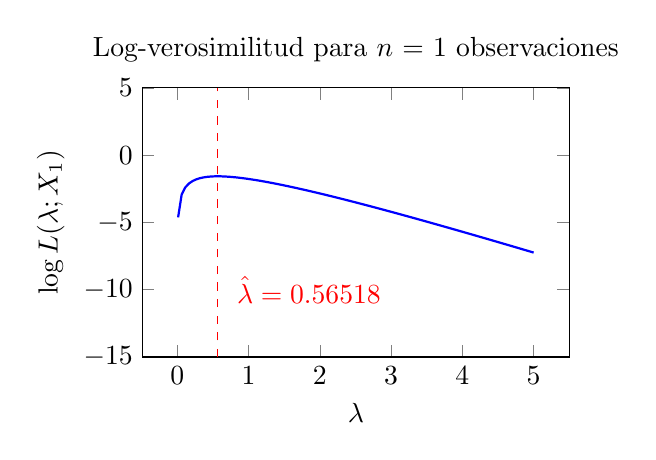
\begin{tikzpicture}
            \begin{axis}[
                    domain=0.01:5,
                    samples=100,
                    ymin=-15, ymax=5,
                    xlabel={$\lambda$},
                    ylabel={$\log L(\lambda; X_1)$},
                    title={Log-verosimilitud para $n$ = 1 observaciones},
                    width=7cm, height=5cm
                ]
                \addplot[thick,blue] {ln(x) - x*1.769362};
                \addplot[red, dashed] coordinates {(0.56518, -15) (0.56518, 5)};.
                \node at (axis cs: 0.7, -10) [anchor=west, red] {$\hat{\lambda} = 0.56518$};
            \end{axis}
        \end{tikzpicture}

    \end{minipage}
    \hfill
    \begin{minipage}{0.48\textwidth}
        \centering

        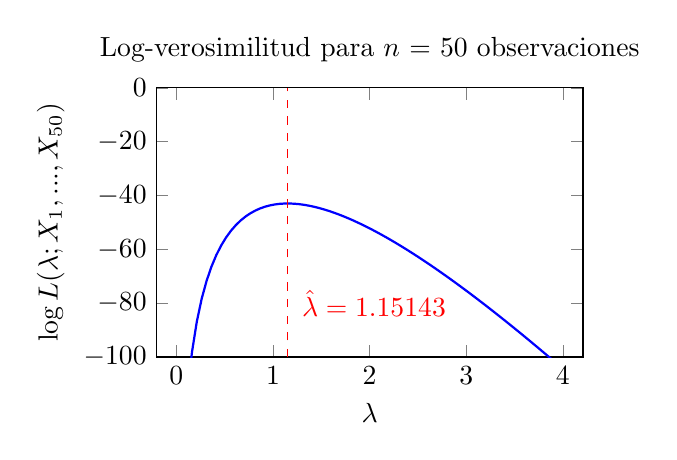
\begin{tikzpicture}
            \begin{axis}[
                domain=0.01:5,
                samples=100,
                ymin=-100, ymax=0,
                xlabel={$\lambda$},
                ylabel={$\log L(\lambda; X_1,...,X_{50})$},
                title={Log-verosimilitud para $n$ = 50 observaciones},
                width=7cm, height=5cm
                ]
                \addplot[thick,blue] {50*ln(x) - x*43.42423};
                \addplot[red, dashed] coordinates {(1.15143, -100) (1.15143, 0)};
                \node at (axis cs: 1.2, -80) [anchor=west, red] {$\hat{\lambda} = 1.15143$};
            \end{axis}
        \end{tikzpicture}

    \end{minipage}

    \begin{center}

        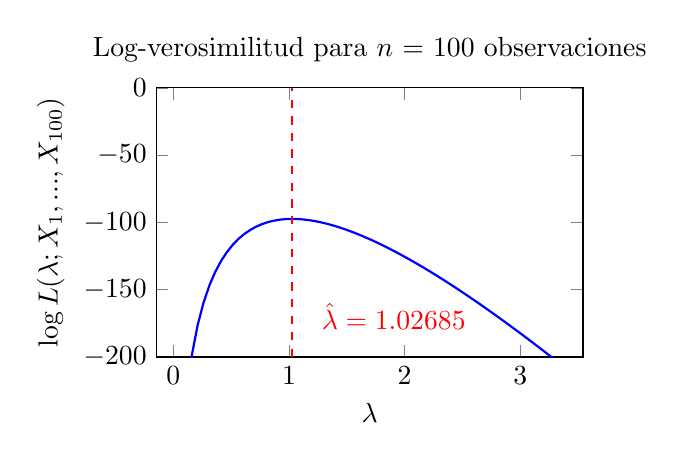
\begin{tikzpicture}
            \begin{axis}[
                domain=0.01:5,
                samples=100,
                ymin=-200, ymax=0,
                xlabel={$\lambda$},
                ylabel={$\log L(\lambda; X_1,...,X_{100})$},
                title={Log-verosimilitud para $n$ = 100 observaciones},
                width=7cm, height=5cm
                ]
                \addplot[thick,blue] {100*ln(x) - x*97.38531};
                \addplot[red, dashed] coordinates {(1.02685, -200) (1.02685, 0)};
                \node at (axis cs: 1.2, -170) [anchor=west, red] {$\hat{\lambda} = 1.02685$};
            \end{axis}
        \end{tikzpicture}
        \caption{Podemos observar como el EMV aproxima el verdadero valor de $\lambda$ en función de la cantidad de observaciones (en este caso $\exp(\lambda)$ donde $\lambda = 1$)}

    \end{center}
    \label{fig:exp-log-ver}
\end{figure}

En la siguiente página se mostrará un ejemplo de como calcular el estimador máximo verosimil de una distribución Bernoulli de parametro $\theta$.

\newpage

\begin{exercise}
    Sean $X_1,\dots,X_n$ v.a.i.i.d. donde $X_i \thicksim B(\theta)$ para $\theta \in (0,1)$. Sea la función de distribución Bernoulli $P_\theta(X=x)=\theta^x(1-\theta)^{1-x}$. Estimar $\theta$ mediante máxima verosimilitud. \\
    Calculamos la verosimilitud como
    \[
        L(\theta;X) \propto \prod_{i=1}^{n}\theta^x(1-\theta)^{1-x}=\theta^{\sum_{i=1}^{n}x_i}(1-\theta)^{n-\sum_{i=1}^{n}x_i}
    \]
    y la log verosimilitud
    \[
        l(\theta; X_1,\dots,X_n)=\sum_{i=1}^{n}x_i\log\theta + (n-\sum_{i=1}^{n}x_i)\log(1-\theta)
    \]
    Encontraremos un máximo en donde se cumpla que $\frac{\partial}{\partial\theta}l(\theta;X_1,\dots,X_n)=0$
    \[
        \frac{\partial}{\partial\theta}l(\theta;X_1,\dots,X_n) = \frac{\sum_{i=1}^{n}x_i}{\theta}-\frac{n-\sum_{i=1}^{n}x_i}{(1-\theta)} \implies
    \]
    \[
        \implies \sum_{i=1}^{n}x_i(1-\theta)=(n-\sum_{i=1}^{n}x_i)\theta \implies \theta=\frac{\sum_{i=1}^{n}x_i}{n}=\overline{X}
    \]
    Por tanto concluimos que el EMV de $\theta$ es $\hat{\theta}=\overline{X}$.
\end{exercise}

\vspace{30pt}

Hilando con la figura \ref{fig:exp-log-ver} donde vemos representada la log verosimilitud de una exponencial, se pondrá como ejemplo también el cálculo del EMV de una distribución exponencial censurada negativa de parámetro $\lambda$.

\textbf{\textit{Definición: }} Sean $X_1, \dots, X_n$ v.a.i.i.d. que siguen una distribución exponencial. Se considera como censura a la derecha cuando se desconoce el tiempo exacto de fallo para $k$ observaciones, pero si se sabe que ocurrió después de un tiempo $t_0$. Es decir, que para $k$ observaciones solo sabemos que $x_i > t_0$.

\vspace{30pt}

Se resolverá el ejercicio en la siguiente página...

\newpage

\begin{exercise}
    Sean $X_1, \dots, X_n$ v.a.i.i.d. donde $X_i$ sigue una exponencial negativa censurada a la derecha de parámetro $\lambda$. Sea la función de distribución exponencial $f(x;\lambda)=\lambda e^{-\lambda x}$. Estimar $\lambda$ mediante máxima verosimilitud. \\
    La función de verosimilitud tendrá dos tipos de datos, los que se obtienen de la exponencial ($f_\lambda(x;\lambda)$) y los $k$ censurados ($P(X_i>t_0)$). \\
    Entonces la función de verosimilitud queda de la siguiente forma:
    \[
        L(\lambda; x_1,\dots,x_n)=\left(\prod_{i=1}^{k}\lambda e^{-\lambda x_i}\right)\left(\prod_{i=k+1}^{n}P(X_i>t_0)\right)
    \]
    Sabemos que
    \[
        P(X_i>t_0)=\int_{t_0}^\infty \lambda e^{-\lambda x}dx = e^{-\lambda t_0}
    \]
    Por lo tanto
    \[
        L(\lambda;x_1,\dots,x_n)=\lambda^k e^{\lambda \sum_{i=1}^{k}x_i}e^{-\lambda(n-k)t_0}
    \]
    Y la log verosimilitud queda
    \[
        l(\lambda;x_1,\dots,x_n)=k\log\lambda-\lambda\left(\sum_{i=1}^{k}x_i + (n-k)t_0\right)
    \]
    Que encontrará máximo en $\hat{\lambda} = \frac{k}{\sum_{i=1}^{k}+(n-k)t_0}$
\end{exercise}

Como último ejemplo se hará lo mismo con la distribución Poisson

\begin{exercise}
    Sean $X_1, \dots, X_n$ v.a.i.i.d. donde $X_i$ sigue una Poisson de parámetro $\lambda$. Sea la función de distribución Poisson $P_\lambda(X=x)=\frac{e^{-\lambda}\lambda^x}{x!}$. Estimar $\lambda$ mediante máxima verosimilitud y comprobar si el estimador es CAN y AE. \\
    La verosimilitud quedará como
    \[
        L(\lambda;x_1,\dots,x_n)=\prod_{i=1}^{n}\frac{e^{-\lambda}\lambda^{x_i}}{{x_i}!}
    \]
    siendo la log verosimilitud
    \[
        l(\lambda; x_1,\dots,x_n)=-n\lambda+\sum_{i=1}^{n}x_i\log\lambda
    \]
    Que encontrará máximo en $\hat{\lambda}=\overline{X}$ \\
    Haciendo uso de este último resultado, es fácil comprobar que $\hat{\lambda}$ es CAN y AE pues
    \[
        \sqrt{n}(\hat{\lambda}-\lambda)=\sqrt{n}(\overline{X}-\lambda) \overset{L}{\to}N(0,\frac{1}{I_1(\lambda)})
    \]
    \[
        I_1(\lambda)=\frac{1}{\lambda} \implies \sqrt{n}(\overline{X}-\lambda)\overset{L}{\to}N(0,\lambda)\square
    \]
\end{exercise}

\newpage

Como generalización del anterior resultado se enuncia el siguiente teorema

\begin{theorem}
    Sean $X_1,\dots,X_n$ v.a.i.i.d. con función de densidad $f(x;\theta)$ donde $\theta \in \Theta$ que verifica CRCR y además que
    \[
        \exists \frac{\partial^3}{\partial \theta^3}\log f(x;\theta) \quad \text{y} \quad \left|\frac{\partial^3}{\partial \theta^3}\log f(x;\theta)\right| \leq M(X); \quad E(M(X))<\infty
    \]
    Entonces el EMV de $\theta$ es CAN y AE. Es decir
    \[
        \sqrt{n}(\hat{\theta}(X)-\theta)\overset{L}{\to}N(0,\frac{1}{I_1(\theta)})
    \]
\end{theorem}

Pongamos un ejemplo

\begin{exercise}
    Sean $X_1, \dots, X_n$ v.a.i.i.d. donde $X_i$ sigue una Normal de parámetros $(0,\sigma^2)$ donde $\sigma^2=\theta$. Sea la función de distribución Normal $f(x;\theta)=\frac{1}{\sqrt(2\pi\theta)}e^{\frac{-x^2}{2\theta}}$. Entonces
    \[
        L(\theta;x_1,\dots,x_n)=\frac{1}{\sqrt{\theta}}e^{\frac{-\sum_{i=1}^{n}x^2_i}{2\theta}} \implies l(\theta;x_1,\dots,x_n)=-\frac{n}{2}\log\theta - \frac{\sum_{i=1}^{n}x^2_i}{2\theta}
    \]
    Que encontrará máximo en $\hat{\theta}=\frac{\sum_{i=1}^{n}x^2_i}{n}$. Entonces
    \[
        \sqrt{n}\left(\frac{\sum_{i=1}^{n}x^2_i}{n}-\theta\right)\overset{L}{\to}N\left(0,\frac{1}{I_1(\theta)}\right)
    \]
    \[
        I_1(\theta)=Var\left(-\frac{n}{2\theta}+\frac{\sum_{i=1}^{n}x^2_i}{2\theta^2}\right)=\frac{n}{2\theta^2}
    \]
    por tanto
    \[
        \sqrt{n}\left(\frac{\sum_{i=1}^{n}x^2_i}{n}-\theta\right) \overset{L}{\to}N(0,2\theta^2) = N(0,2\sigma^4)
    \]
\end{exercise}

Se podría hacer también para una Normal $N(0,\sigma)$ donde $\hat{\theta}=\sqrt{\frac{\sum_{i=1}^{n}x^2_i}{n}}$ que es el EMV para $\sigma$ en modelos $N(0,\sigma)$
Queda como ejercicio para el lector comprobar si

\[
    \sqrt{n}\left(\sqrt{\frac{\sum_{i=1}^{n}x^2_i}{n}}-\sigma\right)\overset{L}{\to}N\left(0,\frac{1}{I_1(\sigma)}\right)
\]
\newpage
\subsubsection{Intervalos de confianza y contrastes de hipótesis uniparamétricos}

Ya hemos visto como estimar el EMV en el caso uniparamétrico. Ahora vamos a ver como se hacen los intervalos de confianza y los contrastes de hipótesis.

\hspace{-1cm}\noindent\begin{tabular}{r}
    \textbf{Ejemplo}  \\ \hline \ \\
\end{tabular}\\
Sean $X_1\dots X_n\sim B(\theta)$ con $0<\theta < 1$, $f(x,\theta)=\theta^x(1-\theta)^{1-x}$, $E(X)=\theta$\ y\ \ $Var(X)=\theta(1-\theta)$

Recordemos que el EMV para $X\sim B(\theta)$ es $\hat\theta_n=\overline{X}$
$$I_1(\theta)=-E\Big(\frac{\partial^2}{\partial\theta^2}ln(f(x,\theta))\Big)=\frac{\theta^2-2\theta^2+\theta}{\theta^2(1-\theta)^2}=\frac{1}{\theta(1-\theta)}$$

Por lo tanto: 
$$\sqrt{n}(\overline{X}-\theta)\overset{\mathcal{L}}{\longrightarrow}N\big(0,\theta(1-\theta)\big)$$

Usando esta distribución asintótica podemos construir \textbf{intervalos de confianza} para $\theta$.
$$P_\theta\Bigg(\underbrace{\frac{\sqrt{n}|\overline{X}-\theta|}{\sqrt{\theta(1-\theta)}}}_{N(0,1)}<\zeta_{1-\frac{\alpha}{2}}\Bigg)=1-\alpha$$

Buscamos el cuantil $\zeta_{1-\frac{\alpha}{2}}$ que hace que la probabilidad sea $1-\alpha$
$$P_\theta\Bigg(-\zeta_{1-\frac{\alpha}{2}}<\frac{\sqrt{n}(\overline{X}-\theta)}{\sqrt{\theta(1-\theta)}}<\zeta_{1-\frac{\alpha}{2}}\Bigg)=1-\alpha$$

Utilizamos la información de Fischer $I_n(\theta)=\frac{n}{\theta(1-\theta)}$ para depejar $\theta$
$$P_\theta\Bigg(-\zeta_{1-\frac{\alpha}{2}}<\frac{(\overline{X}-\theta)}{\sqrt{\frac{1}{I_n(\theta)}}}<\zeta_{1-\frac{\alpha}{2}}\Bigg)=1-\alpha$$
$$P_\theta\Bigg(\overline{X}-\zeta_{1-\frac{\alpha}{2}}\sqrt{\frac{1}{I_n(\theta)}}<\theta<\overline{X}+\zeta_{1-\frac{\alpha}{2}}\sqrt{\frac{1}{I_n(\theta)}}\Bigg)=1-\alpha$$

    \textit{\textbf{Definición:}} La \textbf{Información de Fischer observada }se traduce en sustituir la información de Fischer esperada por su EMV. Como $\hat\theta_n$ es CAN para $\theta$, se tiene que
    $$If_{obs}\overset{p}{\longrightarrow}If_{esp}$$

\noindent En nuestro caso particular consiste en reemplazar $I_n(\theta)=\frac{n}{\theta(1-\theta)}$ por $I_n(\hat\theta)=\frac{n}{\overline{X}(1-\overline{X})}$, luego:
$$P_\theta\Bigg(\overline{X}-\zeta_{1-\frac{\alpha}{2}}\sqrt{\frac{\overline{X}(1-\overline{X})}{n}}<\theta<\overline{X}+\zeta_{1-\frac{\alpha}{2}}\sqrt{\frac{\overline{X}(1-\overline{X})}{n}}\Bigg)=1-\alpha$$

Este tipo de inferencia basada en la verosimilitud se llama \textbf{inferencia de Wald}.\\

Para los contrastes de hipótesis vamos a definir tres estadísticos que nos sirven para hacer inferencia basada en la verosimilitud.
\begin{enumerate}
    \item \textbf{Estadístico de Razón de Verosimilitud}\\\ \\
    Definamos $\lambda (X)$
    $$\lambda (X)=\lambda (X_1,\dots ,X_n)=\Lambda (X)=\frac{L(\theta_0, X_1,\dots,X_n)}{\underset{\theta}{sup}\ L(\theta,X_1,\dots,X_n)}=\frac{L(\theta_0, X_1,\dots,X_n)}{L(\hat\theta_n, X_1,\dots,X_n)}\in [0,1]$$
    $H_0$ se rechazará para valores bajos del estadístico. 
    Ahora vamos a hallar la \textbf{región crítica del test} $\lambda (X)<k$. Para hacerlo más sencillo, se puede escribir con la log-verosimilitud:
    $$Q_L=-2ln(\lambda (X))=-2\big(ln(L(\hat\theta_n,X_1\dots,X_n))-ln(L(\theta_0,X_1\dots,X_n))\big)$$
    En este caso, se rechazará $H_0$ para valores grandes. La región crítica del test será $Q_L>C$. 
    Necesitamos conocer la distribución asintótica de $Q_L$, algo que veremos más adelante.

    \item \textbf{Estadístico de Wald}\\\ \\
    Bajo las condiciones de regularidad de Cramer-Rao podemos escribir $ln(L(\theta_0,X))$ como \textbf{desarrollo de Taylor} en torno a $\hat\theta_n$ como:
    $$ln(L(\theta_0,X))\approx ln(L(\hat\theta_n,X))+(\theta-\hat\theta_n)\overbrace{\frac{\partial}{\partial\theta}ln(L(\hat\theta_n,X))}^{0}+\frac{(\theta-\hat\theta_n)^2}{2}\frac{\partial^2}{\partial\theta^2}ln(L(\hat\theta_n,X))$$
    Recordemos que $\hat\theta_n$ es el EMV, y por tanto el valor de su primera derivada es nula, pero el valor de su segunda derivada no tiene por qué serlo.
Ahora:
    $$Q_L=-2\big(ln(L(\hat\theta_n,X))-ln(L(\theta_0,X))\big)=-2(ln(L(\theta_0,X))+\frac{(\theta-\hat\theta_n)^2}{2}\frac{\partial^2}{\partial\theta^2}ln(L(\hat\theta_n,X))-ln(L(\theta_0,X)))=$$
    $$=-2\Big(\frac{(\theta-\hat\theta_n)^2}{2}\frac{\partial^2}{\partial\theta^2}ln(L(\hat\theta_n,X))\Big)=(\theta-\hat\theta_n)^2\Big(\underbrace{-\frac{\partial^2}{\partial\theta^2}ln(L(\hat\theta_n,X))}_{\text{I. de Fischer observada}}\Big)=$$
    $$=(\theta-\hat\theta_n)^2I_n(\theta)=\frac{n(\theta-\hat\theta_n)^2}{Var(\hat\theta_n)}=Q_W\longleftarrow\text{ \textbf{Estadístico de Wald}}$$
    $Q_L$ y $Q_W$ son asintóticamente equivalentes.

    \item \textbf{Estadístico de Rao}\\\ \\
    $$Q_R=R=\frac{\overbrace{\frac{\partial}{\partial\theta}ln(L(\theta_0,X))}^{\text{Score}}}{I_n(\theta)}$$
    Habíamos visto que 
    $$ln(L(\theta_0,X))\approx ln(L(\hat\theta_n,X))+\frac{(\theta-\hat\theta_n)^2}{2}I_n(\theta)$$
    Ahora vamos a calcular el desarrollo de Taylor para la función score en un entorno de $\hat\theta_n$
    $$S(\theta_0)\approx \underbrace{S(\hat\theta_n)}_{0}+(\theta_0-\hat\theta_n)\frac{\partial^2}{\partial\theta^2}ln(L(\hat\theta_n,X))$$
    \textit{(A partir de este punto el profesor hace una demostración que no es correcta, por lo que he preferido no incluirla, aunque las conclusiones que hay a continuación sí son validas)}\\\ \\
    Este resultado demuestra que $Q_R$ es asintóticamente equivalente a $Q_W$ y $Q_L$. 
\end{enumerate}

Los tres estadísticos rechazarán $H_0$ para valores grandes. Para ver qué distribución siguen, usamos $Q_W$.\\
Sabemos que un EMV es CAN y AE, por lo que:
$$\sqrt{n}(\hat\theta_n-\theta)\overset{\mathcal{L}}{\longrightarrow}N\Big(0,\frac{1}{I_1(\theta)}\Big)\text{ y }\frac{\sqrt{n}(\hat\theta_n-\theta)}{\sqrt{\frac{1}{I_1(\theta)}}}\overset{\mathcal{L}}{\longrightarrow}N(0,1)$$

$Q_W$ es $\displaystyle\frac{\sqrt{n}(\hat\theta_n-\theta)}{\sqrt{\frac{1}{I_1(\theta)}}}$ al cuadrado, por lo que, despejando, se obtiene que:
$$n(\theta-\hat\theta_n)^2I_1(\theta)\overset{\mathcal{L}}{\longrightarrow}\chi^2_1$$
En este punto es conveniente recordar que si una variable $Z\sim N(0,1)$ su cuadrado $Z^2\sim \chi^2_1$

Las distribuciones exactas de $Q_L$, $Q_W$ y $Q_R$ son diferentes, pero como las tres son \textbf{asintóticamente equivalentes}, tenderán a seguir una distribución $\chi^2_1$. 
Por tanto, para determinar el valor de la región crítica solo habría que calcular el siguiente percentil:
$$P_{\theta}(Q_i>c)\approx 1-\alpha\Longrightarrow  c=\chi^2_{1,1-\alpha}$$

\subsection{Caso multiparamétrico}

Situacion:

\(
X_1,\dots,X_n \quad i.i.d. \quad P_\theta,\theta \in \Theta \subseteq \mathbb{R}^s  \text{El parámetro s-dimensional es } \theta = (\theta_1,\dots,\theta_s), \\ \quad s \geq 1
 \text{ con familia de densidad }\{ f(x,\theta),\theta_0 \in \Theta\}
\)

Igualmente podemos escribir

\begin{itemize}
    \item Función de verosimilitud: $L(\theta,X_1,\dots,X_n)=\prod^{n}_{i=1} f(x_i,\theta)$
    \item Función de log-verosimilitud: $l(\theta,X_1,\dots,X_n)=\sum^{n}_{i=1} \log f(x_i,\theta)$
    \item Vector/función score: $$S(\theta,X_1,\dots,X_n)=S(X,\theta)=\frac{d}{d \theta} \log L(\theta,X)
    = \left(\frac{d}{d \theta} \log L(\theta_1,X),\dots,\frac{d}{d \theta} \log L(\theta,X)\right)$$
\end{itemize}

Ahora nos preguntamos, ¿cual es la cantidad de información de Fisher que tendremos en el caso multiparamétrico?.
Para averiguarlo recurrrimos a la matriz Hessiana, que recordamos que es la matriz s x s de las derivadas parciales de segundo orden

\[
I_{ij}(\theta)=E_\theta\left(-\frac{d^2}{d \theta_i d \theta_j} log L(\theta,X)\right)
=E(\frac{d}{d \theta_i} log L(\theta,X),\frac{d}{d \theta_j} log L(\theta,X))
\]
\[
H(\theta,X)=\left\{ \frac{d^2}{d \theta_i d \theta_j}log L(\theta,X) \right\}^s 
=
\begin{pmatrix}
    \frac{d^2}{d \theta_1^2}log L(\theta,X) & \dots & \frac{d^2}{d \theta_1 d \theta_s}log L(\theta,X) \\
    \vdots & \ddots & \vdots \\
    \frac{d^2}{d \theta_s d \theta_1}log L(\theta,X) & \dots & \frac{d^2}{d \theta_s^2}log L(\theta,X)
\end{pmatrix}
\]

Sabiendo esto, $I(\theta)$,matriz de información esperada(que recordemos que es la matriz de covarianzas del vectir score) será:
\[
I(\theta) = E_\theta(-H(\theta,X))
\]
Además de esto tendremos tambíen la matriz de información de Fisher observada

\subsubsection{EMV en el caso multiparamétrico}

$\hat{\theta}=\hat(\theta_n)=(\hat(\theta_1),\dots,\hat(\theta_s))'$ es el EMV para $\theta=(\theta_1,\dots,\theta_s)$
si es la solución al siguiente sistema de ecuaciones:

\[
\begin{matrix}
    \frac{d}{d \theta_1} log L(\theta,X)=0 \\
    \dots \\
    \frac{d}{d \theta_s} log L(\theta,X)=0
\end{matrix}
\]

Estas ecuaciones son las denominadas \textbf{ecuaciones de verosimilitud}.

\subsubsection*{Propiedades asintóticas del EMV multiparamétrico}

En la situación $X_1,\dots,X_n$ i.i.d. $P_\theta, \theta \in \Theta \subseteq \mathbb{R}^s s\geq1$
y bajo las siguientes condiciones de regularidad:

\begin{enumerate}
    \item $\Theta$ es un intervalo de $\mathbb{R}^s$
    \item El soporte de f no depende de $\theta$. $\{x:f(x,\theta)>0\}$ no depende de $\theta$.
    \item $\frac{d}{d \theta_j} f(x,\theta)$ existe y es finita $\forall j=1,\dots,s \quad \theta \in \Theta$
    \item La matriz de información de Fisher (IF($\theta$)) es definida positiva \[ (si \quad \forall X \neq A, \quad X^T \cdot A \cdot X >0) \]
    \item $f(x,\theta) \,dx$ se puede derivar bajo el signo integral
\end{enumerate}
\newpage
Siendo $\theta_0$ el verdadero valor del parámetro, se obtienen los siguientes resultados:

\begin{enumerate}
    \item $P_\theta(L(\theta_0,X)\geq L(\theta,X),\quad \forall \theta \in \Theta) \xrightarrow[n \to \infty]{L}1$
    
    Con probabilidad que tiende a 1, cuando la función de verosimilitud alcanza el máximo en el verdadero valor del parámetro
    \item $\hat{\theta_n} \to \theta_0$. El estimador es consistente.
    \item $\hat{\theta_n} \sim N_s(\theta_0,V(\theta))$ donde $V(\theta)=I^{-1}(\theta)$ (es la inversa de la información de Fisher esperada).
    \item Para una componente de $\hat{\theta_k}$ de $\hat{\theta}$ (vector) se tiene que $\hat{\theta_k} \sim N(\theta_{0k},V_{kk}(\theta))$
    donde $V_{kk}(\theta)$ es el k-ésimo elemento de la diagonal de $V(\theta)$
\end{enumerate}

\subsubsection*{Ejemplo}
\(
Para \quad X_1,\dots,X_n \quad N(\mu,\sigma) 
\)
Obtener $I(\theta)$ esperada

\[
f(x,\mu,\sigma)=\frac{1}{\sigma \sqrt{2 \pi}} \cdot e^{\frac{-(x-\mu)^2}{2 \cdot \sigma^2}}
\]\[ L(\mu,\sigma,X_1,\dots,X_n)= \left(\frac{1}{\sigma \sqrt{2 \pi}}\right)^n \cdot e^{\frac{-1 \cdot \sum_{i=1}^{n}(x_i-\mu)^2}{2 \cdot \sigma^2}}
\]\[ \log L(\mu,\sigma,X_1,\dots,X_n)= -n \log \sigma \cdot \frac{-1}{2 \cdot \sigma^2} \sum_{i=1}^{n}(x_i-\mu)^2
\]

Sacamos las ecuaciones de verosimilitud:
\[
\begin{matrix}
    \frac{d}{d \mu} \log L(\mu,\sigma,X_1,\dots,X_n)=\frac{\sum_{i=1}^{n} (x_i-\mu)}{\sigma^2}=0 \\
    \frac{d}{d \sigma} \log L(\mu,\sigma,X_1,\dots,X_n)=\frac{-n}{\sigma}+ \frac{\sum_{i=1}^{n}(x_i-\mu)^2}{\sigma^3}=0
\end{matrix}
\]
\[
I(\mu,\sigma)=
\begin{pmatrix}
    \frac{n}{\sigma^2} & 0\\
    0 & \frac{2n}{\sigma^3}
\end{pmatrix}
\quad I^{-1}(\mu,\sigma)=
\begin{pmatrix}
    \frac{\sigma^2}{n} & 0\\
    0 & \frac{\sigma^3}{2n}
\end{pmatrix}
\]

luego:

\[
EMV=
\begin{pmatrix}
    \bar{\mu}\\
    \bar{\sigma}
\end{pmatrix}
\sim N_2
\begin{pmatrix}

\begin{pmatrix}
    \bar{\mu_0}\\
    \bar{\sigma_0}
\end{pmatrix}
,
\begin{pmatrix}
    \frac{\sigma^2}{n} & 0\\
    0 & \frac{\sigma^3}{2n}
\end{pmatrix}
    
\end{pmatrix}
\]

o tambien se puede escribir como

\[ EMV=\sqrt{n}
\begin{bmatrix}
    \begin{pmatrix}
        \bar{\mu}\\
        \bar{\sigma}
    \end{pmatrix}
    -
    \begin{pmatrix}
        \bar{\mu_0}\\
        \bar{\sigma_0}
    \end{pmatrix}
\end{bmatrix}
\to
N_2
\begin{pmatrix}
    0,
    \begin{pmatrix}
        \sigma^2 & 0\\
        0 & \frac{\sigma^3}{2}
    \end{pmatrix}
        
    \end{pmatrix}
\]

\subsubsection*{Ejemplo 2:}
Sea $X_1,\dots,X_n$ i.i.d. de una distribución que toma valores en un conjunto finito de valores x=$\{a1,a2,a3\}$ con probabilidad
$P_i$ tal que $\sum_{i=1}^{3} P_i=1$, obtener el EMV.

Se trata de un modelo biparamétrico ya que $P_3=1-P_1-P_2$. $\theta=(P_1,P_2)'$

Función de probabilidad=$f(x; \theta) = P_1 \mathbf{1}_{x = a_1} + P_2 \mathbf{1}_{x = a_2} + P_3 \mathbf{1}_{x = a_3}$

Función de verosimilitud:
\[L(\theta,X_1,\dots,X_n)=\prod_{i=1}^{n}f(x_i,P_1,P_2)=P_1^{N1}\cdot P_2^{N2} \cdot (1-P_1-p_2)^{N3}
\quad donde \quad N_r=\sum_{i=1}^{n} \mathbf{1}_{x_i=a_r}
\]

Log-verosimilitud=$ \log L(\theta,X)=N_1 \log P_1 + N_2 \log P_2 +N_3 \log P_3$

Ecuaciones de verosimilitud:
\[
\begin{matrix}
    \frac{d}{dP_1} \log L(\theta,X)=\frac{N_1}{P_1}-\frac{N_3}{1-P_1-P_2}=0
    \\ \frac{d}{dP_2} \log L(\theta,X)=\frac{N_2}{P_2}-\frac{N_3}{1-P_1-P_2}=0
    
\end{matrix}
\]

Resolviendo el sistema de ecuaciones obtenemos:

\[
\hat{P_1}=\frac{N_1}{n} \quad \hat{P_2}=\frac{N_2}{n} \quad \hat{P_3}=\frac{N_3}{n}
\]
\[
\begin{pmatrix}
    \hat{p_1} \\
    \hat{p_2}
\end{pmatrix}
\sim
N_2
\begin{pmatrix}
    \begin{pmatrix}
        P_1 \\
        P_2
    \end{pmatrix}
, IF^{-1}
\end{pmatrix}
\]

(Hallar la información de Fisher se deja como tarea para el lector)

\subsubsection{Estimación de la varianza a través de la matriz de Información de Fisher observada}

La matriz de información de Fisher es la negativa de la matriz Hessiana calculada en el EMV, es decir $-H(\hat{\theta},X)$
, de forma que el estimador de $V(\theta)$ es:
\[
\hat{V}=\hat{V(\theta)}=-[H(\hat{\theta},X)]^{-1} \quad donde\quad H(\theta,X)=\frac{d^2}{d \theta_i d \theta_j} \log L(\theta,X)
\]
esto ocurre ya que:
\(
H(\hat{\theta},X) \to H(\theta_0,X)
\\ \hat{\theta} \sim N_s(\theta_0,\hat{V})
\hat{\theta_k} \sim N(\theta_{0_k},\hat{V_{kk}})
\)

En esto nos basaremos para hacer inferencia de Wald con intervalos de confianza y contrastes de hipótesis.

\[
Z \sim N_s(\theta,\Sigma) \to \text{Tipificando nos queda}
\]
\[
(Z-\theta)' \Sigma^-1 (Z-\theta) \sim \chi_s^2
\]
\[
\frac{(Z-\theta)^2}{\sigma} \sim \chi^2_1
\]

\subsection{Inferencia de Wald en el caso multiparamétrico}

Si queremos hacer inferencia para 2 o más parámetros, tenemos:

Sea una particion:
\(
\psi=(\theta_1,\dots,\theta_r) \quad r \leq s \quad, \quad
\psi_0=(\theta_{1_0},\dots,\theta_{r_0}) \quad y \quad 
\Omega=(\theta_{r+1},\dots,\theta_s)
\)

Buscamos contrastar: $H_0:\psi=\psi_0$

El EMV para $\psi$ es $\hat{\psi}=(\hat{\theta_1},\dots,\hat{\theta_r})$.

Bajo $H_0$ según lo visto, $\hat{\psi}\sim N_r(\psi_0,\hat{V_\psi})$
donde $\hat{V_\psi}$ es la matriz de covarianzas de $\hat{\psi}$ que es la matriz rxr superior de $\hat{V(\theta)}$.

El estadístico de Wald en este caso es:
\[
W=(\hat{\psi}-\hat{\psi_0}')[\hat{V_\psi}]^{-1}(\hat{\psi}-\psi_0)\sim\chi^2_r
\]
O lo que es lo mismo, en el caso uniparamétrico:
\[
\frac{(\hat{\theta}-\theta)^2}{\sigma}\sim \chi^2_1
\]

Un test de Wald de nivel $\alpha$ rechazará $H_0$ si $W>C_k\equiv W>\chi^2_{1-\alpha,r}$, es decir, si
$\alpha$ es menor que el p-valor=$P_{\psi=\psi_0}(W>W_{obs})\backsimeq$1 - pchisq($W_{obs}$,r).

La región de confianza para $\psi$ con $1-\alpha$ es una elipse r-dimensional para todos los valores ($W \leq \chi^2_{r,1-\alpha}$) en los que el test no rechaza $H_0$

\[
\text{Región de confianza}(1-\alpha)=\{ \psi_0 /\hat{\psi}-\hat{\psi_0}')[\hat{V_\psi}]^{-1}(\hat{\psi}-\psi_0)=\frac{(\hat{\theta}-\theta_s)^2}{\sigma}\leq\chi^2_r\}
\]

¿Cómo hacemos inferencia para una función del parámetro?
Utilizando el delta método s-variante.

Partimos de la situacion $H_0:g(\theta)=0$.

Si g es una función de $\theta$ tal que g:$\theta \to \mathbb{R}^p \quad p \leq S, \quad g(\theta)=(g_1(\theta),\dots,g_p(\theta))$
y sea $G(\theta)$ la matriz p x s de las primeras derivadas respecto a $\theta$:

\[
G(\theta)=
\begin{pmatrix}
    \frac{d}{d \theta_1} g_1(\theta) & \dots & \frac{d}{d \theta_s} g_1(\theta)\\
    \dots &\dots & \dots \\
    \frac{d}{d \theta_1} g_p(\theta) & \dots &\frac{d}{d \theta_s} g_p(\theta)
\end{pmatrix}
\]

Si $\hat{\theta}$ tiene distribución asintótica ($N_s(\theta_s,V)$)
y $g(\hat{\theta})$ también tiene distribución asintótica ($N_p(g(\theta_0)),G_{pxs}(\theta_0)\cdot V \cdot G(\theta)'$)

\[
W=(g(\hat{\theta})-g(\theta_0))'(G(\hat{\theta})\cdot \hat{V} G(\hat{\theta})')^{-1}(g(\hat{\theta})-g(\theta_0)) \sim \chi^2_p
\]

\subsubsection*{Ejercicio 1}
Se analizan 100 lotes con 10 muestras cada uno $\sum_{i=1}^{100}Y_i=12 \quad Y_1,\dots,Y_{100} \sim B(\theta)$.
\\$\theta$="probabilidad de que la toxina esté presente en el lote"
\\ p="probabilidad de que la toxina esté presente en una muestra individual"

\textbf{Apartado a}.

Nos piden hacer inferencia sobre p, sabiendo que p es función de $\theta$.

\[
P(Y_1=0)=1-\theta=(1-p)^{10} \quad P(Y_i=1)=\theta
\]

Ya que ya tenemos la relación, hacemos inferencia sobre p.

\[
L(\theta,Y_1,\dots,Y_{100})=\prod_{i=1}^{100} \theta^{Y_i}(1-\theta)^{1-Y_i}=\theta^{\sum_{i=1}^{100} Y_i}(1-\theta)^{100-\sum_{i=1}^{100} Y_i}
\]\[ \log L(\theta,Y_1,\dots,Y_{100})=(\sum_{i=1}^{100}Y_i) \log \theta + (100-\sum_{i=1}^{100}Y_i) \log (1-\theta)
\]\[ \frac{d}{d \theta} log L(\theta,Y_1,\dots,Y_{100})= \frac{\sum_{i=1}^{100}Y_i}{\theta} - \frac{100 - \sum_{i=1}^{100}Y_i}{1-\theta}=0
\]

El EMV es invariante por transformación: $EMV \to \hat{\theta}=\bar{Y}$
\[
    p=g(\theta)=1-(1-\theta)^{0.1}\Longrightarrow \hat{p}=g(\hat{\theta})=1-(1-\bar{Y})^{0.1}
\]

\textbf{Apartado b}.

Sabemos que $\hat{\theta}=\bar{Y}$ y que tiene distribución asintóticamente normal.

\[
I_n(\theta)=\frac{n}{\theta(1-\theta)} \quad \hat{\theta}\simeq N(\theta,\frac{1}{I_n(\theta)}) = N(\theta,\frac{\theta(1-\theta)}{n})
\]

Sabiendo esto, ¿cuál será la distribución de p?

\[
\hat{p}=g(\hat{\theta}) \simeq N(g(\theta),\frac{\hat{\theta}(1-\hat{\theta})}{n}\cdot (g'(\theta))^2)
\]

¿Y cual sería un intervalo de confianza de Wald con confianza del 95$\%$ para p?

\[
\hat{p} \pm qnorm(0.975)\sqrt{Var(\hat{p})}
\]

\textbf{Apartado c}.
Calcular el ICRV con confianza 0.95 para p.

$$Q_L \approx Q_W \sim \chi^2_1$$

Usamos la fórmula que sabemos para calcular este intervalo para $\theta$.

\[
ICRV=\{ \theta_0:2[\log L(\hat{\theta},X) - log L(\theta_0,X)] \leq qchisq(0.95,1)\}
\]\[=\{ \theta_0:\log L(\theta_0,X) \geq \log L(\bar{Y},X)-\frac{qchisq(0.95,1)}{2}\}
\]

Como los intervalos de confianza basados en RV son invariantes por transformación, el intervalo de confianza RV para p es:

\[
[1-(1-L)^{0.1},1-(1-M)^{0.1}]
\]

(L y M son los puntos entre los que se cumple que $log L(\theta_0,X) \geq \log L(\bar{Y},X)-\frac{qchisq(0.95,1)}{2}$)

\subsection*{Ejercicio 9}

$X_1,\dots,X_n$ i.i.d. con distribución discreta ($P_1=P(ab),P_2=P(Ab),P_3=P(aB),P_4=P(AB)$).

\[
n=3839, \quad N_1=1997,N_2=904, N_3=906, N_4=n-N_1-N_2-N_3
\]
\[
L(x)=\prod_{i=1}^{n}P(X_i=x_i)=P_1^{N_1}\cdot P_2^{N_2}\cdot P_3^{N_3}\cdot (1-P_1-P_2-P_3)^{n-N_1-N_2-N_3}
\]
\[
log L(p,X_1,\dots,X_n)=1997 \log P_1+ 904 \log P_2+906 \log P_3+32\log(1-P_1-P_2-P_3)
\]
\newpage
Ecuaciones de verosimilitud:

\[
\begin{matrix}
    \frac{d}{d P_1} \log L(P_1, X_1, \dots, X_n) = \frac{1997}{P_1} - \frac{32}{1 - P_1 - P_2 - P_3} = 0 \\[1em]
    \dots \\[1em]
    \frac{d}{d P_3} \log L(P_3, X_1, \dots, X_n) = \frac{906}{P_3} - \frac{32}{1 - P_1 - P_2 - P_3} = 0
\end{matrix}
\]
\[
    \text{Resultado:}\quad \hat{P_1}=\frac{N_1}{n}=\frac{1997}{3834} \quad \hat{P_2}=\frac{N_2}{n}=\frac{904}{3834} \quad \hat{P_3}=\frac{N_3}{n}=\frac{906}{3834}
\]

\textbf{Apartado b.}

Calcular el p-valor para el test de Wald.

¿Como relacionamos nuestros parámetros a $\theta$ para contrastar $H_0$? Tenemos que escribir $H_0$ como una función de $g(\theta)$.

El modelo global tiene 3 parámetros. Bajo $H_0$ depende de 1 parámetro y tiene que haber 2 relaciones (2 funciones).

\[
H_0: \quad P_1=\frac{2+\theta}{4}, \quad P_2=\frac{1-\theta}{4}=P_3, \quad P_4=\frac{\theta}{4}
\]\[g_1(P)=P_2-P_3=0, \quad g_2(P)=P_1+P_2-\frac{3}{4}=0
\]\[H_0:
\begin{pmatrix}
    g_1(P)=0 \\
    g_2(p)=0
\end{pmatrix} \qquad (P=2,s=3) \quad H_0=(g(\theta)=(g_1(\theta),\dots,g_P(\theta)))
\]

Utilizando el delta-método multivariante:

\[
g(\hat{p})\sim N_2(g(P),G_{2x3}(\hat{P})\cdot \hat{Var(P)}_{3x3} \cdot G_{3x2}(\hat{P})')
\]

donde $G(\hat{P})$ es la matriz de derivadas parciales evaluadas en $\hat{P}$

\[
G(\hat{P})=
\begin{pmatrix}
    \frac{d}{d P_1} g_1(P) & \frac{d}{d P_2} g_1(P) & \frac{d}{d P_3} g_1(P) \\
    \frac{d}{d P_1} g_2(P) & \frac{d}{d P_2} g_2(P) & \frac{d}{d P_3} g_2(P) 
\end{pmatrix}
\]
\[
W = \left( g_1(\hat{P}), g_2(\hat{P}) \right)' \cdot \left( G(\hat{P}) \, \hat{\text{Var}}(P) \, G(\hat{P})' \right)^{-1} \cdot \left( g_1(\hat{P}), g_2(\hat{P}) \right) \sim \chi^2_2 \quad \text{(bajo } H_0\text{)}
\]

Recordando:   
\[
\begin{matrix}
    g_1(P)=P_2-P_3=0 \\
    g_2(P)=P_1+P_2-\frac{3}{4}=0
\end{matrix}
\quad
G(\hat{P})=
\begin{pmatrix}
    0 & 1 & -1\\
    1 & 1 & 0
\end{pmatrix}
\]
\[
W = \left( \hat{P_2}-\hat{P_3}, \hat{P_1}+\hat{P_2}-\frac{3}{4} \right)' \cdot \left( G(\hat{P}) \, \hat{\text{Var}}(P) \, G(\hat{P})' \right)^{-1} \cdot 
\left(  \hat{P_2}-\hat{P_3}, \hat{P_1}+\hat{P_2}-\frac{3}{4} \right) \sim \chi^2_2 
\]
\[
\text{p-valor}=P_{H_0}(W \geq W_{obs})=1-pchisq(W_{obs},2)=0.36
\]

Volviendo al caso multiparamétrico.

Situación: $\theta=(\theta_1,\dots,\theta_s) \subseteq \mathbb{R}^s \quad \text{y sea }g:\mathbb{R^s}\to \mathbb{R}^r$

\[
g(\theta)=(g_1(\theta),\dots,g(\theta))'
\quad G(\theta)=
\begin{pmatrix}
    \frac{d}{d \theta_1} g_1(\theta) & \dots &  \frac{d}{d \theta_s} g_1(\theta) \\
    \dots & \dots & \dots \\
    \frac{d}{d \theta_1} g_r(\theta) & \dots &  \frac{d}{d \theta_s} g_r(\theta)
\end{pmatrix}
\]

Se requiere contrastar: $H_0:g(\theta)=0 \quad H_1:g(\theta) \neq 0$.
\\ $H_0$ depende de s-r parámetros libres. Con el delta método podemos llegar a calcular un p-valor basado en el test de Wald

Bajo $H_0$:
\[
g(\hat{\theta})-g(\theta) \sim N_r(0,G(\hat{\theta})\cdot \hat{V}(\hat{\theta})\cdot G(\hat{\theta})')
\]
\[
W=(g(\hat{\theta})\cdot [G(\hat{\theta})\cdot \hat{V}(\hat{\theta})\cdot G(\hat{\theta})']^{-1} \cdot g(\hat{\theta})) \sim \chi^2_r
\]
\[
\text{p-valor}=P_{H_0}(\chi^2_r>W_{obs})
\]

Aunque este test es potente, el test de razón de verosimilitud (RV) es más potente.

\subsection{Test de razón de verosimilitud (RV)}

Situación: $X_1,\dots,X_n$ i.i.d. $P_\theta:\theta \in \Theta \subseteq \mathbb{R}^s$

\(
H_0: \theta \in \Theta_0 \subseteq \Theta \quad H_1: \theta \notin \Theta_0
\)

donde $\Theta_0=\{
    \theta \in \Theta: \theta=(\theta_{1_0},\dots,\theta_{r_0},\theta_{r+1},\theta_s)
\}$

$\Theta$ depende de s parámetros libres. $\Theta_0$ depende de r-s parámetros libres.

El test de razón de verosimilitud (TRV) compara el máximo de la verosimilitud en $H_0$ con el mínimo en el EMV

\[
\Delta(x)=\frac{\sup_{\theta \in \Theta_0} L(\theta,X)}{\sup_{\theta \in \Theta} L(\theta,X)}
\]

El estadístivo test de razón de verosimilitud se escribe habitualmente como $-2 \cdot \log \Delta(x)$.
\[
Q_L(x)=2 \cdot [\log L(\hat{\theta},X)-\log L(\hat{\theta_0},X)]
\]
($\log L(\hat{\theta_0},X)$ ees el EMV de $\theta$ restringido a $\Theta_0$ y que depende de s-r parámetros libres)

$Q_L(x)$ bajo $H_0$ tiene una distribución asintótica $\chi^2_r$.
\begin{itemize}
    \item Si $r=s \to H_0:\theta \in \Theta$ es una hipótesis simple, es decir, no hay parámetros libres bajo $H_0.(dim(\Theta_0)=0)$
    \item Si $r<s \to H_0:\theta \in \Theta_0$ es una hipótesis compuesta ($dim(\Theta_0)=s-r$) con s-r parámetros que pueden tomar varios valores posibles.
\end{itemize}

Vamos a usar la notación de partición que vimos antes.

\[
\theta=(\phi,\lambda) \text{ donde } \phi=(\theta_1,\dots,\theta_r) \quad y \quad \lambda=(\theta_{r+1},\dots,\theta_s)
\]

El contraste es: $H_0:\phi=\phi_0 \quad H_1:\phi \neq \phi_0$

Entonces para maximizar sobre el espacio paramétrico restringido a $\Theta_0$ es una maximización sobre $\lambda$ porque
$\Theta_0=\phi_0=(\theta_{1_0},\dots,\theta_{r_0})$ y $\phi_0$ están restringidos.
$$\sup_{\theta \in \Theta}L(\theta,X)=\sup_\lambda L(\phi_0,\lambda,X)$$
\newpage
Bajo las condiciones de regularidad de Cramer-Rao multiparamétrico, 
$Q_L(X) \sim \chi^2_r$ (bajo $H_0$)
y rechazamos $H_0$ para valores grandes de $Q_L(x)$. El test de razón de verosimilitud rechaza $H_0$ a nivel $\alpha$ si $Q_L(x)>\chi^2_{2-\alpha,r}=qchisq(1-\alpha,r)$.
\[
\text{p-valor} \to P_{H_0}(\chi^2_r>Q_{obs})=1-pchisq(Q_{obs},r)
\]
\subsubsection{Región de confianza de la razón de verosimilitud}

La región de confianza (1-$\alpha$) para $\phi=(\theta_1,\dots,\theta_r)\in \mathbb{R}^r$ es la colección de valores
$\phi_0=(\theta_{1_0},\dots,\theta_{r_0})$ para los que $H_0:\phi=\phi_0$ no se rechaza a nuvel $\alpha$.
\[
RCRV(1-\alpha)=\{\phi_0 \in \mathbb{R}^r:H_0:\phi=\phi_0\}
\]\[
    =\{\phi_0 \in \mathbb{R}^r:2[\log L(\hat{\theta},X)-\sup \log L(\phi_0,\lambda,X)] \leq qchisq(1-\alpha,r)\}
\]

La región de confianza de la razón de verosimilitud será un elipsoide r-dimensional. Con s=2 se puede representar.

\textbf{Caso particular para r=1:}

Intervalo de confianza para $\theta_1$ basado en RV con $\theta=(\theta_1,\dots,\theta_s)$ y $\phi=\phi_0$.
\[
ICRV(\theta_1,1-\alpha)=
\]\[\{\theta_{1_0}:H_0:\theta_1=\theta_{1_0}\}
= \left\{ \theta_{1,0} : 2\left[\log L(\hat{\theta},X) - \sup \log L(\phi_0, \lambda, X)\right] \leq qchisq(1 - \alpha, r) \right\}
\]

Buscamos el intervalo de confianza para el caso s=2, es decir, intervalo de confianza para $\theta_1$ con $\phi_0=\theta_1$ y $\lambda=\theta_2$.
\[
ICRV(\theta_1,1-\alpha)=
\]\[
=\left\{ 
\theta_{1_0}:h(\theta_{1_0})=\sup_{\theta_2} \log L(\theta_{1_0},\theta_2,X) \geq \log(\hat{\theta},X)-\frac{qchisq(1-\alpha,1)}{2}=d1
\right\}
\]

Podemos representarlo fácilmente si conocemos la función $h(\theta_{1_0})$.
%Se puede añadir gráfico

El resultado con s=2 es:
\[
\theta_{1_0} \in  ICRV(\theta_1,1-\alpha) \Longleftrightarrow \exists \alpha_2 / (\theta_1,\theta_2) \in B
\]
\[
B=\{\theta=(\theta_1,\theta_2):\log L(\theta,X)>d_1\}
\]
\[
d1=\log L(\hat{\theta},X)-\frac{qchisq(1-\alpha,1)}{2}
\]
%Se puede añadir gráfico

En general, incluso con tamaños de muestra relativamente grandes, el p-valor del test de razón de verosimilitud no coincide con el de Wald.
Siempre es mejor aproximación el test de razón de verosimilitud, especialmente en r$>$1.
\newpage
\subsubsection*{Ejercicio 6}
(Script de R en el campus)

\(
X_1,\dots,X_n \quad \text{i.i.d. discreta} \quad 7
Y_i=\sum_{j=1}^{50} \mathbf{1}_{x_j=i} \quad i=1,2,3
\)
\(
Y_1=8 \quad Y_2=14 \quad Y_3=28
\)

\textbf{Apartado a.}

Contrastar $H_0: p_2-2\cdot p_1=0 \quad H_1: p_2-\cdot p_1 \neq 0$
con TRV.

Pasos:
\begin{enumerate}
    \item Escribimos la función de verosimilitud
    \item Calculamos el EMV
    \item Calculamos la log-verosimilitud en el EMV
    \item Repetimos los 3 primeros pasos bajo $H_0$
\end{enumerate}

Tenemos $p=(p_1,p_2)$ como vector de parámetros.

\[
L(p,x)=\prod_{i=1}^{50} P_p(X=X_i)=P_1^{N_1}\cdot P_2^{N_2}\cdot (1-P_1-P_2)^{50-P_1-P_2}=P_1^8\cdot P_2^{14} \cdot (1-P_1-P_2)^{28}
\]
\[
l(p,x)=8 \log P_1 +14 \log P_2 +28 \log (1-P_1-P_2)
\]
\[
EMV=\left\{
\begin{array}{l}
    \frac{d}{d p_1} \log L(p,x)=0\\
    \frac{d}{d p_2} \log L(p,x)=0
\end{array}
\right.
\quad \hat{p_i}=\frac{N_i}{n}
\quad
\begin{matrix}
    \hat{p_1}=\frac{8}{50}\\
    \hat{p_2}=\frac{14}{50}
\end{matrix}
\]
\[
Q_L(x)=2[\log L(\hat{p},x)-\sup_{p_2=2\cdot p_1}\log L(p,x)]
\]

EMV bajo $H_0$:

\[
sup_{p_1}(8 \log p_1 +14 \log(2\cdot p_1)+28 \log(1-3\cdot P_1))\implies \hat{p_{1_0}=0.15}
\]
\[
Q_l(x)=Q_{obs} \qquad \text{p-valor=}P_\theta(\chi^2_1 \geq Q_{obs})=0.76
\]

No se rechaza $H_0$





\section{Maximización de la verosimilitud}

En la mayoría de casos el EMV se obtiene de forma explícita. Sin embargo, en muchos casos prácticos la ecuación (o ecuaciones) de verosimilitud son muy complejas.
Por ejemplo, para obtener el EMV en R podemos utilizar la función \textit{optim}. En teoría veremos dos algoritmos distintos: el de \textbf{Newton-Raphson} y el \textbf{algoritmo EM}. 

\subsection{Algoritmo de Newton-Raphson (NR)}

Está basado en la aproximación analítica de la función objetivo vía la aproximación lineal de su derivada. \\

Sean $X_1, X_2,...,X_n$ v.a.i.i.d, con $P_\theta\ \theta\in\Theta\subseteq \mathbb{R}^s$ y $\theta=(\theta_1,...,\theta_s)$ donde la función objetivo es $l(\theta,x)=ln(L(\theta,x))$.
El algoritmo NR busca el máximo de la log-verosimilitud a través de la aproximación de su derivada: 
$$\frac{\partial}{\partial\theta}ln(L(\theta,x))=\Big(\frac{\partial}{\partial\theta_1}ln(L(\theta,x)),...,\frac{\partial}{\partial\theta_s}ln(L(\theta,x))\Big)$$
basada en el desarrollo de Taylor.\\

Partimos de un valor inicial "razonable" del parámetro: $\theta_0$ y aproximamos la función por el desarrollo de Taylor.

$$\frac{\partial}{\partial\theta}ln(L(\theta,x))\approx\frac{\partial}{\partial\theta}ln(L(\theta_0,x))+H(\theta_0,x)(\theta-\theta_0)$$
Siendo $H(\theta_0,x)=\Big{\{}\frac{d^2}{d\theta_i d\theta_j}ln(L(\theta,x))\Big{\}}_{i,j}$ la matriz Hessiana de la función de log-verosimilitud. \\

Este resultado es válido para todo $\theta$ y se deduce:

$$\frac{\partial}{\partial\theta}ln(L(\hat\theta,x))\approx\frac{\partial}{\partial\theta}ln(L(\theta_0,x))+H(\theta_0,x)(\hat\theta-\theta_0)$$

Despejando obtenemos lo siguiente:

$$\hat\theta=\theta_0-H(\theta_0,x)^{-1}\frac{\partial}{\partial\theta}ln(L(\theta_0,x))=\theta^{(1)}$$

Si repetimos k veces el paso anterior llegaremos a $\theta^{(k)}$, por lo que la fórmula de actualización del algoritmo en la siguiente iteración será:

$$\theta^{(k+1)}=\theta^{(k)}-H(\theta^{(k)},x)^{-1}\frac{\partial}{\partial\theta}ln(L(\theta^{(k)},x))$$

Es importante la elección del punto inicial para evitar convergencia a \textbf{óptimos locales}.

\newpage
\subsection{Algoritmo EM (\textit{Expectation-maximization})}

Utilizado en situaciones donde los datos que tenemos se pueden considerar \textbf{incompletos} (censurados). 
Es decir, cuando el experimento tiene dos variables aleatorias $Y$ y $B$ pero solamente se observa $Y=y$. $B$ no se observa y los datos completos serán $X=(Y,B)$. 

Sean $X_1, X_2,...,X_n$ v.a.i.i.d, con $P_\theta\ \theta\in\Theta\subseteq \mathbb{R}^s$ con $X_i=(Y_i,B_i)$ y función de densidad $f(x,\theta)=f(y,b,\theta)$ donde solo $Y_1,...,Y_n$ se observan con función de densidad $g(Y,\theta)$.
En este contexto:
\begin{itemize}
    \item f es la función de densidad de los datos \textbf{completos}.
    \item g es la función de densidad de los datos \textbf{observados}.
\end{itemize}
Ambas densidades dependen de $\theta$ pero la densidad de $X$ depende también de $B$, datos que no hemos observado. En estos casos, el EMV lo obtendremos \textbf{siempre} de los \textbf{datos observados}.
\\

La función de verosimilitud de los datos observados es:
$$L(Y_1,...,Y_n,\theta)= \prod_{i=1}^{n}g(Y_i,\theta)$$ $$ln(L(Y,\theta))=\sum_{i=1}^{n}ln(g(Y_i,\theta))$$ Y el EMV será (como siempre): $\hat\theta=\underset{\theta}{arg\ max}[ln(L(Y,\theta))]$
\\

Sin embargo, hay situaciones en las que es difícil resolver y plantear las ecuaciones de verosimilitud. El algoritmo EM nos permite calcular la función de verosimilitud a partir de los datos completos cuando es complicado hacerlo a partir de los observados.
$$L(X_1,...,X_n,\theta)=L((Y_1,B_1),...,(Y_n,B_n),\theta)=\prod_{i=i}^{n}f(Y_i,B_i,\theta)$$

El algoritmo EM obtiene un valor aproximado del EMV que es el máximo de los datos observados a partir del EMV de los datos completos.

\subsubsection{Desarrollo del algoritmo EM}
Se puede calcular la esperanza de $ln(L(X,\theta))$ condicionada a $Y=y$ dado un valor de $\theta$. A partir de un \textbf{valor inicial} $\theta_0$, el algoritmo establece dos pasos:
\begin{enumerate}
    \item \textbf{Esperanza (expectation):} Calcular $E_{\theta_0}\Big(ln(L(X,\theta))\big/Y\Big)$ y sustituir la probabilidad de los valores no observados por el valor esperado condicionado a lo observado.
    \item \textbf{Maximización (maximization):} Obtener $\theta^{(n)}$ en el punto en el que se alcanza el máximo en la log-verosimilitud habiendo sustituido la expresión anterior.
\end{enumerate} 
Este proceso se repite \textbf{iterativamente} $k$ veces. 
\newpage
\textbf{Ejemplo:}(\textit{Este ejemplo es el de la mixtura de la práctica 3 del laboratorio}.)

Sean:
\begin{align*}
    f_1(Y) &= P_p(Y=y) = 
    \begin{cases}
        1 & \text{si } y=0, \\
        0 & \text{si } y \neq 0
    \end{cases} , \quad y = 0, 1, \dots\\
    f_2(Y) &= P_\lambda(Y=y) = e^{-\lambda} \frac{\lambda^y}{y!}, \quad y = 0, 1, \dots
    \end{align*}   
 \\
Primero obtenemos las fórmulas de adecuación del algoritmo para $p$ y $\lambda$.
\begin{itemize}
    \item Datos observados: $Y_i$
    \item Datos completos: $X_i=(Y_i,B_i)$
    \item $B_i$ son datos NO observados
\end{itemize}
Función de densidad conjunta:
$$ f(x,p,\lambda)=f(y,b,p,\lambda)=\begin{cases}
    p & \text{si } b_i=1\ y\ y_i=0 \\
    (1-p)e^{-\lambda}\frac{\lambda^y}{y!} & \text{si } b_i=0\ y\ y_i \neq 0
\end{cases} $$

$$L(p,\lambda,b,y)\propto\prod_{i=1}^{n}p^{b_i}\Big[(1-p)e^{-\lambda}\frac{\lambda^y}{y!}\Big]^{1-b_i}=p^{\sum b_i}(1-p)^{n-\sum b_i}e^{-\lambda(n-\sum b_i)}\lambda^{\sum y_i(1-b_i)}$$
$$ln(L(p,\lambda,b,y))=ln(p)\sum b_i+(n-\sum b_i)ln(1-p)-\lambda(n-\sum b_i)+ln(\lambda)\sum y_i(1-b_i)$$\\\ \\
\underline{Paso 1, Esperanza:} Dados $p_0$ y $\lambda_0$ sustituir $b_i$ por $E_{p_0,\lambda_0}\Big(B_i\Big/Y_i=y\Big)$:
$$E_{p_0,\lambda_0}\Big(ln(L(p_0,\lambda_0,b,y))\Big/Y_1,...,Y_n\Big)=ln(p)\Bigg[\sum E_{p_0,\lambda_0}\Big(B_i\Big/Y_i=y\Big)\Bigg]+ln(1-p)\Bigg[n-\sum E_{p_0,\lambda_0}\Big(B_i\Big/Y_i=y\Big)\Bigg]$$
$$-\lambda\Bigg[n-\sum E_{p_0,\lambda_0}\Big(B_i\Big/Y_i=y\Big)\Bigg]+ln(\lambda)\Bigg[\sum y_i\Big(1-E_{p_0,\lambda_0}\Big(B_i\Big/Y_i=y\Big)\Big)\Bigg]$$
Si tenemos que $b^*_i=E_{p_0,\lambda_0}\Big(B_i\Big/Y_i=y\Big)$ entonces, haciendo uso de la definición de esperanza y Teorema de Bayes:
$$b^*_i=P\Big(B_i=1\Big/Y=y\Big)(1)+P\Big(B_i=0\Big/Y=y\Big)(0)=P\Big(B_i=1\Big/Y=y\Big)=$$
$$=\frac{P_{p_0,\lambda_0}(B_i=1)P\Big(Y_i=y_i\Big/B_i=1\Big)}{P_{p_0,\lambda_0}(B_i=1)P\Big(Y_i=y_i\Big/B_i=1\Big)+P_{p_0,\lambda_0}(B_i=0)P\Big(Y_i=y_i\Big/B_i=0\Big)}=\begin{cases}
    \frac{p_0}{p_0+(1-p_0)e^{-\lambda_0}} & \text{si } y_i=0 \\
    0 & \text{si }y_i \neq 0
\end{cases}$$
Sea $b^{*}=\sum_{i=0}^{n}b^{*}_i$, al ser $p_0$ y $\lambda_0$ constantes, $b^{*}$ será \textbf{una constante} y tenemos que:
$$E_{p_0,\lambda_0}\Big(ln(L(p_0,\lambda_0,b,y))\Big/Y_1,...,Y_n\Big)=b^{*}ln(p)+(n-b^{*})ln(1-p)-\lambda(n-b^{*})+\sum y_i(1-b^{*})ln(\lambda)$$

\noindent\underline{Paso 2, Maximización:} Una vez tenemos la expresión para la esperanza, derivamos y buscamos el máximo en función de cada una de las variables:
$$\begin{cases}
    \frac{\partial}{\partial p}\ E_{p_0,\lambda_0}\Big(ln(L(p_0,\lambda_0,b,y))\Big/Y_1,...,Y_n\Big)=(...)=\frac{b^{*}}{p}-\frac{n-b^{*}}{1-p}=0\\
    \frac{\partial}{\partial \lambda}\ E_{p_0,\lambda_0}\Big(ln(L(p_0,\lambda_0,b,y))\Big/Y_1,...,Y_n\Big)=(...)=(n-b^{*})+\frac{\sum y_i(1-b_i^{*})}{\lambda}=0
\end{cases}$$

La solución de este sistema serán los valores $p^{(1)}$ y $\lambda^{(1)}$, a partir de los cuales podemos repetir el proceso de forma iterativa.

\textbf{Ejercicio 1.Practica 4:}

Tenemos 2 distribuciones N(0,1) y N(1,0.8). Observamos $Y_i$:
\[
Y_i \sim \left\{
    \begin{matrix}
        N(0,1) & \text{con probabilidad P}\\
        N(1,0.8) & \text{con probabilidad 1-P}
    \end{matrix}
\right.\
\quad
\text{ con P desconocida}
\]

Como los datos son incompletos, no observamos $B_i \sim B(p)$. Los datos completos serían $X=(Y_i,B_i)$ con i=$1,\dots,n$.

Función de densidad para los datos completos:
\[
f(y_i,b_i,p)=\left\{
    \begin{matrix}
        f(y_i,2,p)=P_p(B=1) \cdot f_{Y/B=1}(y_i \cdot p)= p \cdot N(0,1) & \text{si b=1}\\
        f(y_i,2,p)=P_p(B=0) \cdot f_{Y/B=0}(y_i \cdot p)= (1-p) \cdot N(1,0.8) & \text{si b=0}
    \end{matrix}
\right.\
\]
\[
=[p \cdot dnorm(y_i,0,1)]^{b_i} \cdot [(1-p) \cdot dnorm(y_i,1,0.8)]^{1-b_i}
\]
Densidad de los datos observados $Y_i$.
\[
g(Y_i,p)=\sum_{b=0}^{1} f(Y_i,b_i,p)=(p \cdot dnorm(y_i,0,1)) + ((1-p) \cdot dnorm(y_i,1,0.8))
\]
\[
L(p,y)=\prod_{i=1}^{n} g(Y_i,p)=\prod_{i=1}^{n} [(p \cdot dnorm(y_i,0,1)) + ((1-p) \cdot dnorm(y_i,1,0.8))]
\]
\[
log L(p,y)=\sum_{i=1}^{n} \log [(p \cdot dnorm(y_i,0,1)) + ((1-p) \cdot dnorm(y_i,1,0.8))]
\]
\[
\frac{d}{dp} log L(p,y)= \sum_{i=1}^{n} \frac{dnorm(y_i,0,1)-dnorm(y_i,1,0.8)}{(p \cdot dnorm(y_i,0,1)) + ((1-p) \cdot dnorm(y_i,1,0.8))}
\]
\[
\frac{d^2}{dp^2} log L(p,y)= \sum_{i=1}^{n} \frac{-(dnorm(y_i,0,1)-dnorm(y_i,1,0.8))^2}{((p \cdot dnorm(y_i,0,1)) + ((1-p) \cdot dnorm(y_i,1,0.8)))^2}
\]
En general:
\[
\theta_{n+1}=\theta_n
-\frac{f'(\theta_n)}{f''(\theta_n)}\]
\newpage
Dado un valor inicial $P_0$, obtenemos P.
\[
p^{(1)}=p_0-\frac{\frac{d}{dp}\log L(p_0,y)}{\frac{d^2}{dp^2}\log L(p_0,y)}
\]
\[
p^{(k+1)}=p_0-\frac{\frac{d}{dp}\log L(p^{(k)},y)}{\frac{d^2}{dp^2}\log L(p^{(k)},y)}
\]

Aplicamos el Algoritmo EM:

Verosimilitud datos completos:

Paso Esperanza: (Dado un $P_0$ inicial) Solo reemplazamos $b_i$ (desconocido) por su esoeranza condicionada a las observaciones.
\[
E_{p_0}(\log L(p,Y_i,B_i)/Y_1,\dots,Y_n)=(\sum_{i=1}^{n} E_{p_0}(B_i/Y_i=y) \log p)
\]\[
+(n-\sum_{i=1}^{n} E_{p_0} E_{p_0}(B_i/Y_i=y) \log (1-p))
\]\[
+\sum_{i=1}^{n} E_{p_0}(B_i/Y_i=y) \log(dnorm(y_i,0,1))+ \sum_{i=1}^{n} ((1-E_{p_0}(B_i/Y_i=y))\cdot \log(dnorm(y_i,1,0.8)))
\]

Necesitamos calcular $E_{p_0}(B_i/Y_i=y)$

\[
B_i=E_{p_0}(B_i/Y_i=y)=1\cdot E_{p_0}(B_i=1/Y_i=y)+0 \cdot E_{p_0}(B_i=0/Y_i=y)
\]
\[
=\frac{p_0 \cdot dnorm(y_i,0,1)}{p_0 \cdot dnorm(y_i,0,1)+(1-p_0)dnorm(y_i,1,0.8)}
\]
Sea $B^*=\sum_{i=1}^{n} B_i^*$:
\[
E_{p_0}(\log L(p,y_i,B_i)/y_i=y_i)=B^* \log p + (n-B^*) \log (1-p) 
\]\[+ \sum_{i=1}^{n} b_i^* \log dnorm(y_i,0,1)
+\sum_{i=1}^{n}(1-b_i^*) \log dnorm(y_i,1,0.8)
\]
\[
\frac{d}{dp} E_{p_0} (\log L(p,Y_i,B_i)/Y_1,\dots,Y_n)=\frac{B^*}{p}-\frac{n-B^*}{1-p}=0
\]
Despejando

\[
p^{(1)}=\frac{B^*}{n}-\frac{1}{n} \sum_{i=1}^{n} \frac{p_0 \cdot dnorm(y_i,0,1)}{p_0 \cdot dnorm(y_i)+(1-p_0)dnorm(y_i,1,0.8)}
\]
\newpage
\textbf{Ejercicio 2.Práctica 4:}




\newpage

% ------------------------------------------------------------------------------
% Reference and Cited Works
% ------------------------------------------------------------------------------

\begin{thebibliography}{9}
    \bibitem{manuscritos}
    Juan Camilo Yepes Borrero, \\ \textit{Apuntes Manuscritos Tema 1}. \\ Universidad de Valladolid 2024.
    \bibitem{apuntes}
    Yolanda Larriba González, \\ \textit{Apuntes INFE2 Tema 1}. \\ Universidad de Valladolid 2023.
\end{thebibliography}

% ------------------------------------------------------------------------------

\end{document}